\documentclass[a4paper,oneside,10pt]{article}

%%%\newenvironment{proof}{\hbox{}\vspace{-0.8cm} {\bf Proof:}}{\hfill $\Box$ \vspace{0.2cm}}

\usepackage{amsmath}
\usepackage{amsthm}
\usepackage{amssymb}
\usepackage{amsfonts}
\usepackage{mathrsfs} 
\usepackage{graphicx}
\usepackage{color,xcolor}
%\usepackage{ulem}
\usepackage{bm}

\usepackage{tikz}
\usetikzlibrary{arrows.meta, positioning}

\usepackage{hyperref}

\usepackage{cleveref}

% --------- ALGORITHMS ---------- <<:
\usepackage{algorithm,algorithmic}
%\usepackage[noend]{algpseudocode}      %%% this is for the algorithms
\renewcommand{\algorithmicrequire}{\textbf{Input:}} % require --> input
\renewcommand{\algorithmicensure}{\textbf{Output:}} % ensure --> output
% :>> ALGORITHMS

\newtheorem{theorem}{Theorem}[section]
\newtheorem{lemma}[theorem]{Lemma}
\newtheorem{proposition}[theorem]{Proposition}
\newtheorem{corollary}[theorem]{Corollary}
%\newtheorem{algorithm}[theorem]{Algorithm}
\newtheorem{conjecture}[theorem]{Conjecture}
\newtheorem{condition}[theorem]{Condition}
\newtheorem{definition}[theorem]{Definition}
\newtheorem{assumption}[theorem]{Assumption}
\newtheorem{remark}[theorem]{Remark}
\newtheorem{problem}[theorem]{Problem}
\newtheorem{example}[theorem]{Example}
\newtheorem{notation}[theorem]{Notation}
\usepackage{booktabs}

\usepackage{geometry}
\geometry{
 a4paper,
 %total={170mm,257mm},
 left=30mm,
 right=30mm,
 top=30mm,
 bottom=30mm
}

%\textheight235mm
%\textwidth165mm
%\voffset-10mm
%\hoffset-12.5mm
\parindent0.8cm
\parskip0mm


\usepackage{stmaryrd} %for double brackets

%\usepackage{mathptmx}

% updates

\newcommand{\R}{\mathbb{R}} % real numbers
\newcommand{\C}{\mathbb{C}} % complex numbers
\newcommand{\N}{\mathbb{N}} % integers
\newcommand{\allmat}{\mathbb{M}} % matrices
\newcommand{\sym}{\mathbb{S}} % matrices symétriques
\newcommand{\PP}{\mathcal{P}}
\newcommand{\Qc}{\mathcal{Q}}
\renewcommand{\span}[1]{{\text{span}(#1)}} % simone's comments
\newcommand{\aff}[1]{{\text{aff}(#1)}} % simone's comments
\newcommand{\relint}[1]{{\text{relint}(#1)}} % simone's comments
\newcommand{\calL}{\mathcal{L}} % simone's comments

\newcommand{\simone}[1]{{\color{blue} #1}} % simone's comments
\newcommand{\corentin}[1]{{\color{red} #1}} % corentin's comments
\newcommand{\tristan}[1]{{\color{red} #1}} % tristan's comments
\newcommand{\todo}[1]{{\color{blue}\bf \text{TODO: } #1}} % TODOs

%p-adic commands
\DeclareMathOperator{\val}{val}
\def\QQ{\ensuremath{\mathbb{Q}}}
\def\ZZ{\ensuremath{\mathbb{Z}}}
\newcommand{\OK}{\mathcal{O}_K}
\def\diag{\mathrm{diag}}

\newcommand{\GL}{\mathrm{GL}}

\newcommand{\exend}{\hfill $\blacksquare$}


\usepackage{biblatex}
\addbibresource{../rapport/bibstage.bib}

\title{\Large \bf On semidefinite-representable sets over valued fields}

\begin{document}

\author{Corentin Cornou$^{1}$, Simone Naldi$^{2}$ and Tristan Vaccon$^{2}$}

\footnotetext[1]{ENS Paris-Saclay, Université Paris-Saclay, France.}
\footnotetext[2]{Université de Limoges, CNRS, XLIM, UMR 7252, F-87000 Limoges, France.}
%\footnotetext[3]{Sorbonne Université, CNRS, LIP6, Equipe PolSys, F-75005 Paris, France.}

\date{Draft of \today}

\maketitle

\begin{abstract}
  \noindent
  Real polyhedra and real spectrahedra (or their projections) are respectively the feasible sets
  of linear and semidefinite programming, and form the family of
  semidefinite-representable sets. This paper investigates versions of these sets and of
  the related optimization problems with data over a valued field $K$.
  For $K$-polyhedra and linear programming over $K$ we give an algorithm based on computation
  of Smith normal forms.
  We prove that basic properties of semidefinite-representable sets generalize to this setting.
  In particular, we showcase examples of non-polyhedral $K$-spectrahedra and of sets that are
  semidefinite representable over $K$ but are not $K$-spectrahedra.
\end{abstract}

%\tableofcontents

\section{Introduction}

The study of polyhedra and of linear programming (LP) is at the heart of convex geometry and optimization, inasmuch as several optimization problems can be cast as, or relaxed to LP. An important generalization of LP is semidefinite programming (SDP), namely the problem of minimizing a linear function over the set of positive semidefinite affine combinations of some real symmetric matrices. The latter problem has interested the community of real algebraic geometry and polynomial optimization, mostly because of the relaxation method known as moment-SOS (or Lasserre) hierarchy \cite{henrion2020moment}.

The main motivation for studying the effective aspects of SDP is the fact that, despite several properties of LP extend to SDP, the complexity status of SDP is, contrary to the LP case, widely open. Ramana's construction \cite{ramana1997exact} implies a series of general results: in the Blum-Shub-Smale real numbers machines model \cite{blum1989theory}, the feasibility of SDP is in $\text{NP} \cap \text{co-NP}$, whereas it is not known to be in NP in the Turing model; checking boundedness, attainability and optimality can be polynomially reduced to the feasibility of SDP \cite{ramana1997exact}. Assuming the input data belongs to an effective field $K$ (\emph{e.g.} $K = \QQ$) then a solution can be described and computed as element of a vector space over some algebraic extension of $K$. For exact computation, complexity bounds are known based either on general quantifier elimination \cite{ramana1997exact,porkolab1997complexity} and explicit algorithms exist based on a dedicated application of the so-called critical point method, and exploiting the determinantal structure of the constraints \cite{henrion2016exact,NALDI2018206}. A complexity analysis for the computation of an approximate solution of an SDP can be made based on the ellipsoid algorithm \cite{khachiyan1979polynomial,grotschel1981ellipsoid} or on interior-point methods \cite{de2016turing}; in this approximation framework, SDP is solvable in polynomial time in the input size (\emph{i.e.} matrix size, number of variables, bit size of the coefficients), $\log(\frac{1}{\varepsilon})$ (where $\varepsilon$ is the target precision) and $\log(\frac{R}{r})$, where $r,R$ are radii of balls respectively included in and containing the feasible set, cf. \cite{grotschel1981ellipsoid} or \cite[Thm.1.1]{de2016turing} (see also \cite[Sec.1.9]{deKlerk}).

In this paper we consider the situation where input data are defined over fields $K$ with a prescribed valuation map $\val$ on $K$. In this context a polyhedron is defined as a set of vectors such that some linear forms have nonnegative or infinite vluation ({\it cf.} \Cref{def_polyhedra}). The prototype of valued field we target is the field of $p$-adic numbers with $p$-adic valuation.
%%%\todo{Give motivations for p-adic precision of LP/SDP.}
Similar generalizations have been recently proposed in the context of tropical geometry \cite{iriarte2022polyhedral} and tropical methods applied to non-archimedean semidefinite programming \cite{allamigeon2016solving,allamigeon_tropical_2020}.

%\subsection{Context and motivations}
%Il faudra entre autre mentionner (et peut être motiver l'approche p-adique) :
%\begin{itemize}
%\item les questions ouvertes de complexité concernant la programmation semidefinie (pas clair si NP $\cap$ co-NP
%  dans le modele de Turing)
%\item les questions ouvertes géométriques (Conjecture de Lax)
%\end{itemize}
%\subsection{Main results}


%\newpage
\section{Preliminaries}

Throughout the paper, $(K,\val)$ refers to a complete valued field, namely $K$ is a field
and $\val : K \twoheadrightarrow \Gamma \cup \{+\infty\}$ is a valuation on $K$, $\Gamma$ an
ordered abelian group. The valuation is often assumed to be discrete ({\it i.e.} $\Gamma=\ZZ$)
with $\pi \in K$ a uniformizer. The ring of integers of $K$ is
$$
\OK = \{x \in K : \val(x) \geq 0\},
$$
$\kappa = \OK/\mathfrak{m}_K$ its residue field, with
$\mathfrak{m}_K = \{x \in K : \val(x) > 0\}$.
For $k \in \N$, we write $O(\pi^k)$ for $\pi^k \OK$.
A typical example of $K$ as above is the field of $p$-adic numbers 
$\QQ_p$ equipped with the $p$-adic valuation. For this example, we 
have $\OK = \ZZ_p$. Another example is the field of Laurent series
$K=\QQ(\!(t)\!)$ equiped with $t$-adic valuation,
in which case $\OK = \QQ \llbracket t \rrbracket$.
We refer to \cite{Serre:1979,engler2005valued} for a
general introduction to such fields
and to \cite{caruso_computations_2017}
for an introduction to effective computations over $p$-adic numbers.

The $K$-vector space of polynomials of degree $\leq d$ on $x=(x_1,\ldots,x_n)$
with coefficients in $K$ is denoted by $K[x]_{d}$. The ring of matrices of
size $p \times q$ with entries in a ring $R$ is $R^{p \times q}$ and the general
linear group in $R^{n \times n}$ is $\GL_n(R)$.
For the sake of ease of writing, block-diagonal matrices with blocks
$B_1,\ldots,B_d$ are denoted by $\diag(B_1, \ldots, B_d)$, the null matrix of
size $p \times q$ by ${\bf 0}_{p,q}$, and the identity matrix by $I_t$.

We recall the definition of Smith Normal Form, in our context.
\begin{definition}[Smith Normal Form]\label{smith_nf}
  Assume $(K,\val)$ is a discrete valued field with uniformizer $\pi$.
  Let $M \in K^{m \times n}$ be of rank $r$. There exist unique integers
  $a_1 \leq \cdots \leq a_r$, and
  matrices $P \in \GL_n(\OK)$ and $Q \in \GL_m(\OK)$, such that
  $$
  \mathrm{SNF}(M) := QMP^{-1} = \diag(\pi^{a_1}, \pi^{a_2}, \ldots, \pi^{a_r}, {\bf 0}_{m-r,n-r}).
  $$
  The matrix $\mathrm{SNF}(M)$ is called the \emph{Smith Normal Form (SNF)} of $M$, and the elements $\pi^{a_i}$ the
  \emph{invariant factors}.
\end{definition}
\begin{remark}
  The valuation of the first invariant factor of $\mathrm{SNF}(M)$ of a matrix
  $M \in K^{n \times n}$ is the minimum of the valuations of the entries of
  $M$. In particular, $\mathrm{SNF}(M) \in \OK^{n \times n}$.
\end{remark}

Let us now give a short introduction to classical ({\it i.e.} real) polyhedra and spectrahedra.
Let $\sym_d(\R) \subset \R^{d\times d}$ be the vector space of $d \times d$ real symmetric
matrices. A matrix $M \in \sym_d(\R)$ is \emph{positive semidefinite} ($M \succeq 0$) whenever the quadratic form $x \mapsto x^TMx$ is nonnegative for all $x\in \R^n$. By the Spectral Theorem, $M \succeq 0$ if and only if the eigenvalues of $M$ are nonnegative, and this is equivalent to all the principal minors of $M$ being nonnegative. The set $\sym_d^+(\R) \subset \sym_d(\R)$ of positive semidefinite matrices is a closed convex cone with non-empty interior in $\sym_d(\R)$.

Let $A_0,A_1,\ldots,A_n \in \sym_d(\R)$, and let $\calL = A_0+\span{A_1,\ldots,A_n}$ be the affine space
containing $A_0$ and with direction the vector space spanned by $A_1,\ldots,A_n$ (which we might assume
to be linearly independent). The intersection
$$
\calL \cap \sym_d^+(\R) = \left\{A(x) := A_0+\sum_i x_i A_i \in \sym_d(\R) :
A(x) \succeq 0\right\},
$$
or equivalently, its pre-image $S = \{x \in \R^n : A(x) \succeq 0\}$ under the map $x \mapsto A(x)$, is called
a \emph{real spectrahedron}. As (linear preimage of) affine sections of $\sym_d^+(\R)$, real spectrahedra
are closed convex sets, but might have empty interior in $\calL$ (resp. in $\R^n$).
Moreover, they are basic semialgebraic sets, indeed they are defined by sign conditions on the principal
minors of the defining matrix as well as sign conditions on the coefficients of its characteristic polynomial
(cf. \Cref{ell3}).

\begin{example}\label{ell3}
  Let $d=n=3$. The $3$-elliptope is the three-dimensional spectrahedron given by
  $$
  \mathcal{E}_3 :=
  \left\{
  x
  \in \R^3 :
  \begin{bmatrix}
    1 & x_1 & x_2 \\
    x_1 & 1 & x_3 \\
    x_2 & x_3 & 1
  \end{bmatrix}
  \succeq 0
  \right\}
  =
  \left\{
  x
  \in \R^3 :
  \begin{array}{r}
    3-x_1^2-x_2^2-x_3^2 \geq 0 \\
    1+2x_1x_2x_3-x_1^2-x_2^2-x_3^2 \geq 0
  \end{array}
  \right\}.
  $$
  The polynomials on the right are the (non-constant) coefficients of the univariate polynomial
  $p(t) = \det(A(x)+t I_3)$,
  whose roots are the opposites of the eigenvalues of the defining matrix. Equivalently $\mathcal{E}_3$
  is defined by positivity of the principal minors of the defining matrix:
  $$
  1-x_1^2 \geq 0, \,\,\, 1-x_2^2 \geq 0, \,\,\, 1-x_3^2 \geq 0 \,\,\, \text{ and } \,\,\, 1+2x_1x_2x_3-x_1^2-x_2^2-x_3^2 \geq 0.$$ \exend
\end{example}

The optimization problem of miminizing a linear function over a real spectrahedron is called \emph{semidefinite programming} (SDP).
%Given $c \in \R^n$ and $A_0,A_1,\ldots,A_n \in \sym_d(\R)$, the corresponding semidefinite program is defined (in standard dual form) as
%\begin{equation}
%  \label{SDP}
%\begin{array}{rcll}
%  p^* & := & \inf_{x \in \R^n} & \left\langle c, x \right\rangle \\
%  &    & \text{s.t.}         & A_0+\sum_{i=1}^n x_i A_i \succeq 0.
%\end{array}
%\end{equation}
{\it Real polyhedra} (subsets of $\R^n$ defined by finitely many affine inequalities) are special cases of real
spectrahedra, where the defining matrices $A_0, \ldots, A_n$ can be chosen diagonal, so that
$A = \diag(\ell_1,\ldots, \ell_d)$. In other words, SDP is a generalization of Linear Programming (LP).

% IN INTRODUCTION
%In a fixed-precision model of computation, SDP is solvable in polynomial time in the input size (matrix size,
%number of variables, bit size of the coefficients), in $\log(\frac{1}{\varepsilon})$ (where $\varepsilon$ is the
%precision) and $\log(\frac{1}{R})$, where $R$ is an {\it a priori} upper bound on the norm of a solution,
%cf. \cite[Sec.1.9]{deKlerk}. In exact arithmetic, the complexity status of SDP is essentially open but complexity
%bounds are known based either on general quantifier elimination \cite{ramana1997exact,porkolab1997complexity}
%or by exploiting the determinantal structure of the constraints \cite{henrion2016exact}.

A more general class of convex semialgebraic sets are obtained by linear projections of real spectrahedra
called \emph{semidefinite representable sets}: these are sets of the form
$$
P = \left\{x = \left[\begin{smallmatrix} x_1 \\ \vdots \\ x_n \end{smallmatrix}\right] \in \R^n : \exists\,y\in\R^m, \, A_0 + \sum_{i=1}^n x_i A_i + \sum_{j=1}^m y_j B_j \succeq 0\right\}.
$$
When $m>0$, the set $P$ is also called a \emph{spectrahedral shadow}.

\begin{example}
\label{fermat_quartic}
The basic closed semialgebraic set $P = \{(x_1,x_2) \in \R^2 : 1-x_1^4-x_2^4 \geq 0\}$ is not a spectrahedron
but it is semidefinite representable:
$$
P = \left\{\begin{bmatrix} x_1 \\ x_2 \end{bmatrix} \in \R^2 :
\exists\,
\begin{bmatrix} y_1 \\ y_2 \end{bmatrix} \in \R^2, \,
\diag\left(
\begin{bmatrix}
  1+y_1 & y_2 \\
  y_2 & 1-y_1
\end{bmatrix},
\begin{bmatrix}
  1 & x_1 \\
  x_1 & y_1
\end{bmatrix},
\begin{bmatrix}
  1 & x_2 \\
  x_2 & y_2
\end{bmatrix}
\right)
\succeq 0
\right\}
$$
\end{example}


\section{Polyhedra}

In this section, we define polyhedra over a complete discrete valued field $K$ with valuation $\val$ and a uniformizer $\pi$, and we prove that the class of polyhedra is closed under linear transformations, as in the real case. We end by presenting an algorithm for solving linear optimization problems over $K$.

\begin{definition}
  \label{def_polyhedra}
  A \emph{polyhedron} is a subset $P \subset K^n$ of the form
  $$
  P = \{x \in K^n : \val(\ell_i(x)) \geq 0, i=1,\ldots,d \text{ and }
  \val(m_j(x)) = +\infty, j=1,\ldots,e\},
  $$
  for some $\ell_1,\ldots,\ell_d,m_1,\ldots,m_e \in K[x]_1$.
\end{definition}

%%We recall that that the smallest affine space of $K^n$ containing a set $S \subset K^n$ is called its \emph{affine hull} and denoted $\aff{S}$. The assumption on forms $\ell_i$ in \Cref{def_polyhedra} implies that the constraint $\val(m_1 \oplus \cdots \oplus m_e) = +\infty$ defines exactly the affine hull of $P$, in other words $\aff{P} = \{x \in K^n : m_j(x) = 0, j=1,\ldots,e\}$ \simone{(il nous faudrait une preuve, du genre: $\val(m(x))=+\infty$ pour tout $x \in P$ si et seulement si $m$ est une combinaison affine de $m_1,\ldots,m_e$.)}
%%The \emph{dimension} of $P$ is defined as the dimension of $\aff{P}$ (for $e=0$, $\aff{P}=K^n$ and $P$ has dimension $n$). The \emph{relative interior} of $P$ is defined as $\relint{P} = \{x \in P : \val(\ell_1 \oplus \cdots \oplus \ell_d) < +\infty\}$ (\simone{pas clair si besoin de dimension et relint}).
Remark that \Cref{def_polyhedra} includes the case $d=0$ corresponding to affine spaces, as in the real case.
Moreover by definition the class of polyhedra is closed under intersection. Without loss of generality, one may
assume in \Cref{def_polyhedra} that for every $i=1,\ldots,d$ there exists $x \in P$ such that
$\val(\ell_i(x))<+\infty$.

\begin{example}
  The \emph{closed unit ball} $\OK^n=B_\infty(K^n)$ in $K^n$ for the supremum norm $||\cdot||_{\infty}$ is the
  polyhedron defined as the set of $x=(x_1,\ldots,x_n) \in K^n$ such that $||x||_{\infty} =
  \max_i\{x_i\} \leq 1$, in other words, such that $\val(x_i) \geq 0$, for all $i=1, \ldots, n$.
  In other words, $\OK^n$ is the polyhedron in $K^n$ defined by the affine polynomials
  $\ell_i(x)=x_i$, $i=1,\ldots, n$, and $e=0$. %%%%%(its affine hull is indeed the whole $K^n$).
\end{example}

\subsection{Projections and direct image of polyhedra}

%{\color{blue} Normalement avec la nouvelle definition, ça devrait aller, il faut par contre
%  partir d'un polyedre defini aussi par des égalités. Peut être il faudrait aussi
%  diviser la proposition en plusieures parties pour la rendre plus lisible, par exemple une
%  première proposition avec la projection.}

In this section, we prove that the class of polyhedra is stable
by applying affine maps:

\begin{theorem}[DI] 
Let $f : K^n \to K^m$ be an affine map and $\PP$ a polyhedron of $K^n.$
Then $f(\PP)$ is a polyhedron. \label{theo:DI}
\end{theorem}

We prove the result by reducing to particular cases.
The strategy to deduce the main theorem DI 
is the following:
\begin{figure}[htbp]
\centering
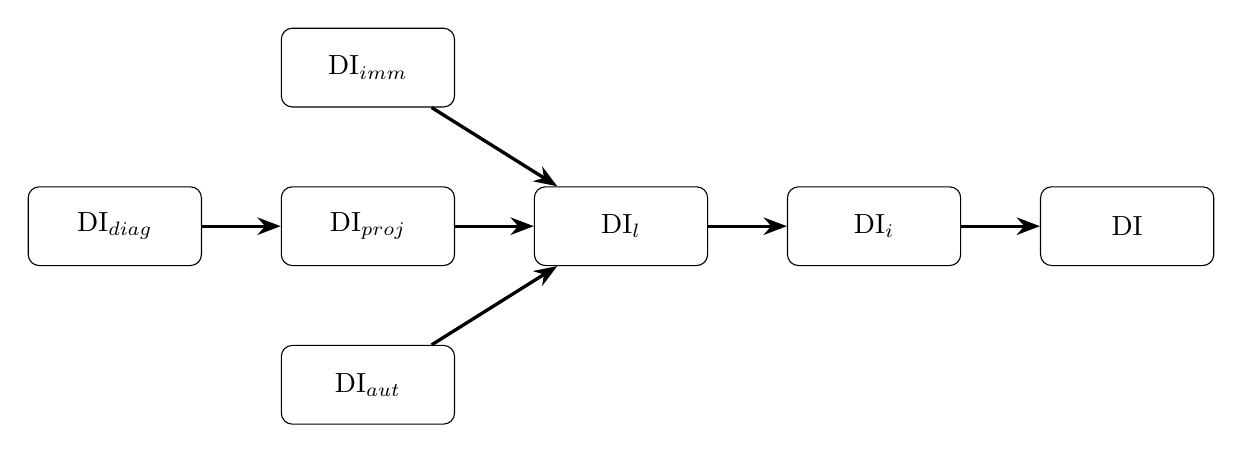
\begin{tikzpicture}[
  node distance=1cm and 1cm,
  box/.style={draw, rounded corners, minimum width=2.2cm, minimum height=1cm, align=center},
  thickarrow/.style={->, >=Stealth, line width=1.2pt},
]

% Nodes
\node[box] (DIdiag) {DI${}_{diag}$};
\node[box, right=of DIdiag] (DIproj) {DI${}_{proj}$};
\node[box, right=of DIproj] (DIl) {DI${}_{l}$};
\node[box, right=of DIl] (DIi) {DI${}_{i}$};
\node[box, right=of DIi] (DI) {DI};

\node[box, above=of DIproj] (DIimm) {DI${}_{imm}$};
\node[box, below=of DIproj] (DIaut) {DI${}_{aut}$};

% Arrows
\draw[thickarrow] (DIdiag) -- (DIproj);
\draw[thickarrow] (DIproj) -- (DIl);
\draw[thickarrow] (DIl) -- (DIi);
\draw[thickarrow] (DIi) -- (DI);

\draw[thickarrow] (DIimm) -- (DIl);
\draw[thickarrow] (DIaut) -- (DIl);

\end{tikzpicture}
\caption{Strategy of proof of Theorem \ref{theo:DI}.}
\label{fig:di-properties}
\end{figure}



We begin by the cases of linear maps in $GL_n(O_K)$.

\begin{lemma}[DI${}_{aut}$]
Let $f \in GL_n(O_K)$ and $\PP$ a polyhedron of $K^n$.
Then $f(\PP)$ is a polyhedron. \label{lem:DIaut}
If in addition, $\PP$ is defined only by inequalities,
then so is $f(\PP)$.
\end{lemma}
\begin{proof}
If $\PP$ is defined (in matrix form) by \[\left\lbrace X \in K^n,  AX+B \geq 0, CX+D=0 \right\rbrace\] and $U$ is the matrix of $f$ in the canonical basis of $K^n$, 
let $\Qc$ be defined by \[\left\lbrace Y \in K^n,  AU^{-1} Y+B \geq 0, CU^{-1} Y+D=0 \right\rbrace.\]
Then it is clear that $\Qc$ is a polyhedron and $f(\PP)=\Qc.$
It is also clear that if $\PP$ is defined only by inequalities,
then so is $f(\PP)$.
\end{proof}

If $f$ is diagonal, we can also conclude.

\begin{lemma}[DI${}_{diag}$]
Let $f : K^n \to K^n$ be a linear map and $\PP$ a polyhedron of $K^n$ defined only by inequalities. We assume that the matrix of $f$ in the canonical basis of $K^n$ is diagonal.
Then $f(\PP)$ is a polyhedron. \label{lem:DIdiag}
\end{lemma}
\begin{proof}
As in the proof of Lemma \ref{lem:DIaut} DI${}_{aut}$, a trivial change
of variables is enough to conclude.
\end{proof}


We now treat the case where $f$ is a projection erasing the last coordinate.

\begin{lemma}[DI${}_{proj}$]
Let $f : K^n \to K^n, \: (x_1,\dots,x_{n-1},x_n) \mapsto (x_1,\dots,x_{n-1})$ and $\PP$ a polyhedron of $K^n$ defined only by inequalities. 
Then $f(\PP)$ is a polyhedron defined only by inequalities. \label{lem:DIproj}
\end{lemma}
\begin{proof}
We assume that $\PP \neq \emptyset$.
Let us write the conditions defining $\PP$
in matrix form:
$\val(A X+B) \geq 0$ 
with $A \in M_{q,n}(K)$, $B \in K^q$
and $X=(x_1,\dots,x_n)^\intercal$. 


We can compute a Smith Normal Form
of the $q \times (n-1)$ matrix defined by the 
$n-1$ first columns of $A$
to obtain a decomposition of the form:
\[ Q_A A P_A^{-1} = \begin{bmatrix}
\delta_1	& 		& 			&   &		 &  &a_1	\\
			& \ddots& 			& 0	&		 &	&		\\
			&		& \delta_l  &   & 		 &	&		\\
			&		&			&0  & 		 &	& 		\\
			&		&			&   & \ddots &	&		\\
			&		&			&	&		 & 0&a_{n-1} \\
			&		&			&	&		 &	&a_n 	\\
			&		&			&	&		 &	&    	\\
			&		&			&	&		 &	&a_q 	\\			
\end{bmatrix},\]
with $Q_A \in \GL_q(\OK)$ and $P_A \in \GL_n(\OK)$ such that $P_A(e_n)=e_n.$

Multiplying on the left by $Q_A^{\pm 1}$ does not
modify whether the valuation inequalities are satisfied.
Moreover, thanks to Lemma \ref{lem:DIaut} DI${}_{aut}$,
$\PP$ can be written
$\PP=P_A^{-1}(\PP_2)$ for some polyhedron $\PP_2 \subset K^n$
and we are reduced to proving that
$f(\PP_2)$ is a polyhedron for $p$ the projection
$K^n \rightarrow K^{n-1}$ and $\PP_2$
defined by the following linear matrix inequality (for some $B_2 \in K^q$):
\[  \begin{bmatrix}
\delta_1	& 		& 			&   &		 &  &a_1	\\
			& \ddots& 			& 0	&		 &	&		\\
			&		& \delta_l  &   & 		 &	& \vdots\\
			&		&			&0  & 		 &	& 		\\
			&		&			&   & \ddots &	&		\\
			&		&			&	&		 & 0&a_{n-1} \\
			&		&			&	&		 &	&a_n 	\\
			&		&			&	&		 &	& \vdots   	\\
			&		&			&	&		 &	&a_q 	\\			
\end{bmatrix} \begin{bmatrix} x_1 \\ \\ \\ \\ \\ \vdots \\ \\ \\ \\ x_n \\ \end{bmatrix} + B_2 \geq 0.\]



We remark that 
$a_s x_n + b_s \geq 0$
if and only if $x_n = -a_s^{-1} b_s + O(\pi^{- \val(a_s)}).$
This exactly corresponds to $x_n \in B(-a_s^{-1} b_s,\val(a_s)).$
Since the conditions have to be compatible (we have assumed
$\PP$ not empty), and thanks to ultrametricity,  
the intersection of these conditions for 
$s \in \llbracket l+1,q \rrbracket$
is then given by the smallest of these balls.
Let us assume it is the one defined for $l=n.$
The only condition on $x_n$
is then $\val(a_nx_n +b_n) \geq 0.$

Thanks to Lemma \ref{lem:DIdiag} DI${}_{diag}$,
we can further assume that the $\delta_i$'s and $a_n$ are all $1$'s
and are reduce to $\PP_2$ defined by the linear matrix inequality:
\[  \begin{bmatrix}
1	& 		& 			&   &		 &  &a_1	\\
			& \ddots& 			& 0	&		 &	&		\\
			&		& 1  &   & 		 &	& \\
			&		&			&0  & 		 &	& 	\vdots	\\
			&		&			&   & \ddots &	&		\\
			&		&			&	&		 & 0&a_{n-1} \\
			&		&			&	&		 &	&1 	\\
		
\end{bmatrix} \begin{bmatrix} x_1 \\ \\  \\ \\ \vdots \\  \\ \\ x_n \\ \end{bmatrix} + \begin{bmatrix} b_1 \\ \\ \\  \\ \vdots  \\ \\ \\ b_n \\ \end{bmatrix}  \geq 0.\]
Finally, we can also assume that, up to a permutation of the variables, $\val(a_1)= \min_{i=1}^{n-1} \val(a_i).$
We distinguish two cases: $\val(a_1) \geq 0$ and $\val(a_1)<0.$

Let us first assume that $\val(a_1) \geq 0$.

Let $x \in \PP_2$.
Then $x_n=-b_n+O(1)$
and $x_1+a_1 x_n+b_1=O(1).$
Consequently, $x_1-a_1 b_n +b_1=O(1)+O(\pi^{\val(a_1)})=O(1).$
Similarly, for all $i \in \llbracket 2,n-1 \rrbracket,$
$x_i-a_ib_n+b_i=O(1)+O(\pi^{\val(a_i)})=O(1).$

We define the polyhedron $\Qc \subset K^{n-1}$ by the following inequalities:
 for all $i \in \llbracket 1,n-1 \rrbracket,$
$\val(x_i-a_ib_n+b_i) \geq 0$.

Then the previous computations prove that $p(\PP_2)\subset \Qc.$
Conversely, let $(x_1,\dots,x_{n-1}) \in \Qc.$
Then let $x_n := -b_n.$

We check that for $i \in \llbracket 1,n-1 \rrbracket,$
$x_i+a_ix_n+b_i=x_i-a_ib_n+b_i=O(1),$
and $x_n+b_n=O(1)$. Hence $(x_1,\dots,x_n) \in \PP_2$
which means that $(x_1,\dots,x_{n-1}) \in p(\PP_2).$
Thus $p(\PP_2)= \Qc$ and $p(\PP_2)$ is a polyhedron.

We now deal with the second case, with $\val(a_1)<0.$
Let $x \in \PP_2$.
Then $x_n=-b_n+O(1)$
and $x_1+a_1 x_n+b_1=O(1).$
Consequently, $x_1-a_1 b_n +b_1=O(1)+O(\pi^{\val(a_1)})=O(\pi^{\val(a_1)}).$
Thus $a_1^{-1}x_1- b_n +a_1^{-1}b_1=O(1)$.
%and $x_n=-a_1^{-1}(x_1+b_1)+O(1).$
In addition, $x_n=-a_1^{-1}(x_1+b_1)+O(\pi^{-\val(a_1)}).$
We plug this equality in 
$x_i+a_i x_n+b_i=O(1)$ to get
$x_i-a_1^{-1}a_i(x_1+b_1)+b_i=O(1)+O(\pi^{\val(a_i)-\val(a_1)})=O(1)$
using that $\val(a_i) \geq \val (a_1).$

We define the polyhedron $\Qc \subset K^{n-1}$ by the following inequalities:
$\val(a_1^{-1}x_1- b_n +a_1^{-1}b_1) \geq 0$ and for all $i \in \llbracket 2,n-1 \rrbracket,$
$\val(x_i-a_1^{-1}a_i(x_1+b_1)+b_i) \geq 0.$

Then the previous computations prove that $p(\PP_2)\subset \Qc.$
Conversely, let $(x_1,\dots,x_{n-1}) \in \Qc.$
Let $x_n := -a_1^{-1}(x_1+b_1).$
Then
$x_1+a_1 x_n+b_1=0=O(1).$
Let $i \in \llbracket 2,n-1 \rrbracket,$
then $x_i+a_i x_n+b_i=x_i-a_1^{-1}a_i(x_1+b_1)+b_i=O(1)$
since $(x_1,\dots,x_{n-1}) \in \Qc.$
Finally, 
$x_n+b_n=-a_1^{-1}(x_1+b_1)+b_n=O(1)$ thanks to the inequality satisfied by $x_1.$
Hence $(x_1,\dots,x_n) \in \PP_2$
which means that $(x_1,\dots,x_{n-1}) \in p(\PP_2).$
Thus $p(\PP_2)= \Qc$ and $p(\PP_2)$ is a polyhedron,
and it has been proved in both cases.

Therefore, $p(\PP)$ is a polyhedron (and inequalities are enough to define $p(\PP_2)$ as a polyhedron).
\end{proof}

\begin{lemma}[DI${}_{imm}$]
Let $f : K^l \to K^n$ be the immersion $(x_1,\dots, x_l) \mapsto (x_1,\dots, x_l,0,\dots, 0)$ and $\PP$ a polyhedron of $K^l$
Then $f(\PP)$ is a polyhedron. \label{lem:DIimm}
\end{lemma}
\begin{proof}
Adding the equalities $x_{l+1}=0, \dots, x_n=0$ to the equations and inequations in
$x_1,\dots, x_l$ defining $\PP$, the result is clear.
\end{proof}

We can now generalize to linear mappings and
polyhedron defined only by inequalities.

\begin{proposition}[DI${}_l$]
Let $f : K^n \to K^m$ be a linear map and $\PP$ a polyhedron of $K^n$ defined only by inequalities.
Then $f(\PP)$ is a polyhedron. \label{prop:DIl}
\end{proposition}
\begin{proof}
We assume that $\PP \neq \emptyset$, and we identify $f$ with its matrix in $\allmat_{n,m}(K)$.
We assume that $\PP$ is defined as $\left\lbrace x \in K^n : \val (l_i (x) ) \geq 0, \textrm{ for } i \in I\right\rbrace$ for some
finite sets $I \subset \N$ and $l_i \in K[x]_1$, for $i \in I$ .

Thanks to Definition \ref{smith_nf}, (the matrix of) $f$
can be written $f=Q^{-1} \Delta P$
with $P \in \GL_n(\OK),$ $Q \in \GL_m(\OK)$
and $\Delta = \mathrm{SNF}(f)\in \allmat_{n,m}(K)$ of the form $\diag(\lambda_1, \ldots, \lambda_r, {\bf 0}_{\min(m,n)-r})$
  where ${\bf 0}_{\min(m,n)-r}$ is a null square matrix of size $\min(m,n)-r$ for $\lambda_1,\dots,\lambda_r$ non-zero and $r \in \N.$

By Lemma \ref{lem:DIaut} DI${}_{aut}$,
$P(\PP)$ is a polyhedron defined only by inequalities.

Let $\Qc= P(\PP)$
We now prove that $\Delta (\Qc)$ is a polyhedron.
One can write that $\Delta$ is the composition
of the immersion 
$K^r \rightarrow K^n$
$(x_1,\dots,x_r)\mapsto (x_1,\dots,x_r,0,\dots,0),$ 
 the diagonal invertible mapping
$K^l \rightarrow K^l$,
$(x_1,\dots,x_r)\mapsto (\delta_1,\dots,\delta_r x_r)$,
and the projections
$(x_1,\dots,x_{r+1})\mapsto (x_1,\dots,x_{r}),$
 $(x_1,\dots,x_{r+2})\mapsto (x_1,\dots,x_{r+1}),$
 $\dots,$
 $(x_1,\dots,x_{n})\mapsto (x_1,\dots,x_{n-1}).$
 Thus, thanks to Lemmas \ref{lem:DIimm} DI${}_{imm}$, \ref{lem:DIproj} DI${}_{proj}$ and \ref{lem:DIaut} DI${}_{aut}$, $\Delta (\Qc)$ is a polyhedron.
 One can note that it is only when applying the immersion as the last mapping in the composition chain that equalities are needed to define the last polyhedron.



Finally, thanks to Lemma \ref{lem:DIaut} DI${}_{aut}$,
$Q^{-1} \left( \Delta (\Qc) \right)$ is a polyhedron.
This concludes the proof.
\end{proof}

We can generalize from linear mappings to affine mappings.
\begin{proposition}[DI${}_i$]
Let $f : K^n \to K^m$ be an affine map and $\PP$ a polyhedron of $K^n$ defined only by inequalities.
Then $f(\PP)$ is a polyhedron. \label{prop:DIi}
\end{proposition}
\begin{proof}
Let $P \in K^m$. One can see by immediate change of variables that $\Qc$ is a polyhedron of $K^m$ if and only if
$\Qc+P$ is a polyhedron of $K^m$.
Consequently, translating by $-f(O)$ in the codomain, one can reduce
to the case of Proposition \ref{prop:DIl}   DI${}_l$.
\end{proof}

We can now conclude with the proof of the main result
of this section.

\begin{proof}[Proof of Theorem \ref{theo:DI} DI]
Here, $f : K^n \to K^m$ is an affine map and $\PP$ a polyhedron of $K^n.$
Let us write $\PP = \PP_I \cap \PP_E$
with $\PP_I := \left\lbrace X \in K^n,  AX+B \geq 0 \right\rbrace$
and $\PP_E := \left\lbrace X \in K^n,  CX+D=0 \right\rbrace = P + \overrightarrow{\PP_E}.$ 

Then $f(\PP) = f_{\PP_E}(\PP_I).$

By a translation of $-P$ in $K^n$, we can assume that
$\PP_E$ is a linear vector space: we are reduced to proving that, if $\tilde{f}: \PP_E \to K^m$ is an affine map and $\PP_I$ is a polyhedron of the vector space $\PP_E$ defined only by inequalities, then  $\tilde{f}(\PP_I)$ is a polyhedron.
This is the case thanks to Proposition \ref{prop:DIi} DI$_i$
and the theorem is proven.
\end{proof}



%
%In this section we show that the image of a polyhedron by a linear mapping is a polyhedron,
%and discuss some consequences.
%We first prove the result in the cases of authomorphisms of $\OK^n$ and diagonal endomorphisms of $K^n$.
%Then we use these particular cases to prove the result for projections of the form
%$(x_1,\dots,x_n) \mapsto (x_1,\dots, x_{n-1})$ and finally for the general case.
%
%\begin{remark}
%  Let $f : K^n \to K^m$ be a linear map and let
%  $P = \{x \in K^n : \val(l_i(x)) \geq 0, m_i(x) = 0, 1 \leq i \leq d, 1 \leq j \leq e\}$.
%  Then $P = P_I \cap P_E$ where $P_I := \{x \in K^n : \val(l_i(x)) \geq 0, 1 \leq i \leq d\}$
%  and $P_E := \{x \in K^n : m_j(x) = 0, 1 \leq j \leq e\}$.
%
%  Thus we have\footnote{\simone{Ça n'est pas vrai en général, il faut que $f$ soit injective.
%    Il faut peut être d'abord factoriser $f = g \circ h$ avec $h : K^n \to im(f)$ et
%    $g : im(f) \subset K^m$.}}
%  $f(P) = f(P_I) \cap f(P_E)$. However $P_E$ is either empty or an affine subspace of
%  $K^n$ and therefore $f(P_E)$ is either empty or an affine subspace of $K^m$, so it is a polyhedron.
%  Hence, as the class of polyhedra is closed under intersection, in order to prove that
%  $f(P)$ is a polyhedron, it is sufficient to prove that this holds for $f(P_I)$.
%\end{remark}
%
%Therefore below we consider polyhedra of the form as in \Cref{def_polyhedra} with $e=0$.
%
%\begin{proposition}\simone{l'enoncé est incomplet}
%  Let $P \subset K^n$ be a polyhedron and let $f : K^n \to K^n$ be a linear mapping.
%  If $f \in \GL_n(\OK)$ or if there exists $\lambda_1, \dots, \lambda_n \in K$ such that
%  $(x_1,\dots,x_{n-1}, x_n) \mapsto (x_1,\dots, x_{n-1})$.
%\end{proposition}
%
%\begin{proof}
%We assume that $\PP \neq \emptyset$
%As discussed above we can assume that
%$\PP = \left\lbrace x \in K^n : \val (l_i (x) ) \geq 0,\textrm{ for } i \in I \right\rbrace$ for some
%finite set $I \subset \N$ and $l_i \in K[x]_1$, for $i \in I$ .
%
%First, if $f \in \GL_n(\OK)$ then, $x \in f(P)$ if and only if for all $i \in I$, 
%$\val(l_i (f^{-1}(x))) \geq 0$.
%The $l_i \circ f^{-1}$ are clearly in $K[x]_1$
%and $f(P)$ is a polyhedron.
%
%Similarly, if $f:K^n \rightarrow K^n$ is of the form
%$f(x_1,\dots,x_n)=(\lambda_1 x_1,\dots,\lambda_n x_n)$
%for some $\lambda_1,\ldots, \lambda_n \in K$,
%then of course $f(P)$
%can be defined by $\val (\widetilde{l_i}(x)) \geq 0$, $i \in I$
%with the $\widetilde{l_i}$'s obtained from the $l_i$'s by an
%obvious change of variables.
%\end{proof}
%
%The two above results\footnote{\simone{il y en an un}}
%allows us to demonstrate the following proposition, which we will use to prove the general case. 
%
%\begin{proposition}
%      Let $\PP \subset K^n$ be a polyhedron and $p : K^n \to K^{n-1}$ be the projection $p : (x_1,\dots,x_{n-1},x_n) \mapsto (x_1, \dots, x_{n-1})$.
%       Then $p(\PP)$ is a spectrahedron.
%\end{proposition}
%
%
%\begin{proof}
%      
%We assume that $\PP \neq \emptyset$.
%As discussed above we can assume that
%  $\PP = \left\lbrace x \in K^n : \val (l_i (x) ) \geq 0,\textrm{ for } i \in I \right\rbrace$ for some
%finite set $I \subset \N$ and $l_i \in K[x]_1$, for $i \in I$ .
%
%Let us write the conditions defining $\PP$
%in matrix form:
%$\val(A X+B) \geq 0$ and 
%with $A \in M_{q,n}(K)$, $B \in K^q$
%and $X=(x_1,\dots,x_n)^\intercal$. 
%
%
%We can compute a Smith Normal Form
%of the $q \times (n-1)$ matrix defined by the 
%$n-1$ first columns of $A$
%to obtain a decomposition of the form:
%\[ Q_A A P_A^{-1} = \begin{bmatrix}
%\delta_1	& 		& 			&   &		 &  &a_1	\\
%			& \ddots& 			& 0	&		 &	&		\\
%			&		& \delta_l  &   & 		 &	&		\\
%			&		&			&0  & 		 &	& 		\\
%			&		&			&   & \ddots &	&		\\
%			&		&			&	&		 & 0&a_{n-1} \\
%			&		&			&	&		 &	&a_n 	\\
%			&		&			&	&		 &	&    	\\
%			&		&			&	&		 &	&a_q 	\\			
%\end{bmatrix},\]
%with $Q_A \in \GL_q(\OK)$ and $P_A \in \GL_n(\OK)$ such that $P_A(e_n)=e_n.$
%
%Multiplying on the left by $Q_A^{\pm 1}$ does not
%modify whether the valuation inequalities are satisfied.
%Moreover, thanks to our previous on the case when $f$ is an automorphism,
%$\PP$ can be written
%$\PP=P_A^{-1}(\PP_2)$ for some polyhedron $\PP_2 \subset K^n$
%and we are reduced to proving that
%$f(\PP_2)$ is polyhedron for $p$ still the canonical projection
%$K^n \rightarrow K^{n-1}$ and $\PP_2$
%defined by the linear matrix inequality (for some $B_2 \in K^q$):
%\[  \begin{bmatrix}
%\delta_1	& 		& 			&   &		 &  &a_1	\\
%			& \ddots& 			& 0	&		 &	&		\\
%			&		& \delta_l  &   & 		 &	& \vdots\\
%			&		&			&0  & 		 &	& 		\\
%			&		&			&   & \ddots &	&		\\
%			&		&			&	&		 & 0&a_{n-1} \\
%			&		&			&	&		 &	&a_n 	\\
%			&		&			&	&		 &	& \vdots   	\\
%			&		&			&	&		 &	&a_q 	\\			
%\end{bmatrix} \begin{bmatrix} x_1 \\ \\ \\ \\ \\ \vdots \\ \\ \\ \\ x_n \\ \end{bmatrix} + B_2 \geq 0.\]
%
%
%
%We remark that 
%$a_s x_n + b_s \geq 0$
%if and only if $x_n = -a_s^{-1} b_s + O(\pi^{- \val(a_s)}).$
%This exactly corresponds to $x_n \in B(-a_s^{-1} b_s, 2^{\val(a_s)}).$
%Since the conditions have to be compatible (we have assumed
%$\PP$ not empty), and thanks to ultrametricity,  
%the intersection of these conditions for 
%$s \in \llbracket l+1,q \rrbracket$
%is then given by the smallest of these balls.
%Let us assume it is the one defined for $l=n.$
%The only condition on $x_n$
%is then $\val(a_nx_n +b_n) \geq 0.$
%
%Thanks to the above discussion on diagonal mapping,
%we can further assume that the $\delta_i$'s and $a_n$ are all $1$'s
%and are reduce to $\PP_2$ defined by the linear matrix inequality :
%\[  \begin{bmatrix}
%1	& 		& 			&   &		 &  &a_1	\\
%			& \ddots& 			& 0	&		 &	&		\\
%			&		& 1  &   & 		 &	& \\
%			&		&			&0  & 		 &	& 	\vdots	\\
%			&		&			&   & \ddots &	&		\\
%			&		&			&	&		 & 0&a_{n-1} \\
%			&		&			&	&		 &	&1 	\\
%		
%\end{bmatrix} \begin{bmatrix} x_1 \\ \\  \\ \\ \vdots \\  \\ \\ x_n \\ \end{bmatrix} + \begin{bmatrix} b_1 \\ \\ \\  \\ \vdots  \\ \\ \\ b_n \\ \end{bmatrix}  \geq 0.\]
%Finally, we can also assume that, up to a permutation of the variables, $\val(a_1)= \min_{i=1}^{n-1} \val(a_i).$
%We distinguish two cases: $\val(a_1) \geq 0$ and $\val(a_1)<0.$
%
%Let us first assume that $\val(a_1) \geq 0$
%
%Let $x \in \PP_2$.
%Then $x_n=-b_n+O(1)$
%and $x_1+a_1 x_n+b_1=O(1).$
%Consequently, $x_1-a_1 b_n +b_1=O(1)+O(\pi^{\val(a_1)})=O(1).$
%Similarly, for all $i \in \llbracket 2,n-1 \rrbracket,$
%$x_i-a_ib_n+b_i=O(1)+O(\pi^{\val(a_i)})=O(1).$
%
%We define the polyhedron $\Qc \subset K^{n-1}$ by the following inequalities:
% for all $i \in \llbracket 1,n-1 \rrbracket,$
%$\val(x_i-a_ib_n+b_i) \geq 0.$
%
%Then the previous computations prove that $p(\PP_2)\subset \Qc.$
%Conversely, let $(x_1,\dots,x_{n-1}) \in \Qc.$
%Then let $x_n := -b_n.$
%
%We check that for $i \in \llbracket 1,n-1 \rrbracket,$
%$x_i+a_ix_n+b_i=x_i-a_ib_n+b_i=O(1),$
%and $x_n+b_n=O(1)$. Hence $(x_1,\dots,x_n) \in \PP_2$
%which means that $(x_1,\dots,x_{n-1}) \in p(\PP_2).$
%Thus $p(\PP_2)= \Qc$ and $p(\PP_2)$ is a polyhedron.
%
%We now deal with the second case, with $\val(a_1)<0.$
%Let $x \in \PP_2$.
%Then $x_n=-b_n+O(1)$
%and $x_1+a_1 x_n+b_1=O(1).$
%Consequently, $x_1-a_1 b_n +b_1=O(1)+O(\pi^{\val(a_1)})=O(\pi^{\val(a_1)}).$
%Thus $a_1^{-1}x_1- b_n +a_1^{-1}b_1=O(1)$.
%%and $x_n=-a_1^{-1}(x_1+b_1)+O(1).$
%In addition, $x_n=-a_1^{-1}(x_1+b_1)+O(\pi^{-\val(a_1)}).$
%We plug this equality in 
%$x_i+a_i x_n+b_i=O(1)$ to get
%$x_i-a_1^{-1}a_i(x_1+b_1)+b_i=O(1)+O(\pi^{\val(a_i)-\val(a_1)})=O(1)$
%using that $\val(a_i) \geq \val (a_1).$
%
%We define the polyhedron $\Qc \subset K^{n-1}$ by the following inequalities:
%$\val(a_1^{-1}x_1- b_n +a_1^{-1}b_1) \geq 0$ and for all $i \in \llbracket 2,n-1 \rrbracket,$
%$\val(x_i-a_1^{-1}a_i(x_1+b_1)+b_i) \geq 0.$
%
%Then the previous computations prove that $p(\PP_2)\subset \Qc.$
%Conversely, let $(x_1,\dots,x_{n-1}) \in \Qc.$
%Let $x_n := -a_1^{-1}(x_1+b_1).$
%Then
%$x_1+a_1 x_n+b_1=0=O(1).$
%Let $i \in \llbracket 2,n-1 \rrbracket,$
%then $x_i+a_i x_n+b_i=x_i-a_1^{-1}a_i(x_1+b_1)+b_i=O(1)$
%since $(x_1,\dots,x_{n-1}) \in \Qc.$
%Finally, 
%$x_n+b_n=-a_1^{-1}(x_1+b_1)+b_n=O(1)$ thanks to the inequality satisfied by $x_1.$
%Hence $(x_1,\dots,x_n) \in \PP_2$
%which means that $(x_1,\dots,x_{n-1}) \in p(\PP_2).$
%Thus $p(\PP_2)= \Qc$ and $p(\PP_2)$ is a polyhedron,
%and it has been proved in both cases.
%
%Therefore,$p(\PP)$ is a polyhedron.
%
%\end{proof}
%
%We can finally prove that the image of polyhedron under a linear mapping is a polyhedron.
%\begin{proposition}
%Let $\PP \subset K^n$ be a polyhedron and $f: K^n \rightarrow K^m$
%be a linear mapping. Then $f(\PP)$ is a polyhedron.
%\end{proposition}
%
%\begin{proof}
%
%We assume that $\PP \neq \emptyset$, and we identify $f$ with its matrix in $\allmat_{n,n}(K)$.
%As seen above, we can assume that $\PP$ is of the form $\left\lbrace x \in K^n : \val (l_i (x) ) \geq 0, \textrm{ for } i \in I\right\rbrace$ for some
%finite sets $I \subset \N$ and $l_i \in K[x]_1$, for $i \in I$ .
%
%Thanks to Definition \ref{smith_nf}, (the matrix of) $f$
%can be written $f=Q^{-1} \Delta P$
%with $P \in \GL_n(\OK),$ $Q \in \GL_m(\OK)$
%and $\Delta = \mathrm{SNF}(f)\in \allmat_{m,n}(K)$ of the form $\diag(\lambda_1, \ldots, \lambda_r, {\bf 0}_{\min(m,n)-r})$
%  where ${\bf 0}_{\min(m,n)-r}$ is a null square matrix of size $\min(m,n)-r$ for $\lambda_1,\dots,\lambda_r$ non-zero and $r \in \N.$
%
%  %Now, we turn our attention to the $\Delta$ part of $f$.
%We have previously proven that if $f \in \GL_n(\OK)$ then $f(\PP)$ is a polyhedron.
%It is also clear that
%if $f$ is the immersion 
%$K^l \rightarrow K^n$
%$(x_1,\dots,x_l)\mapsto (x_1,\dots,x_l,0,\dots,0)$ 
%and $\PP$ is a polyhedron in $K^n$,
%then $f(\PP)$ is a polyhedron.
%
%
%We now prove that for
%$\Delta$ a Smith Normal Form
%and $\PP$ a polyhedron,
%$\Delta(\PP)$ is a polyhedron.
%Then $\Delta$ is the composition
%of the immersion 
%$K^l \rightarrow K^n$
%$(x_1,\dots,x_l)\mapsto (x_1,\dots,x_l,0,\dots,0),$ 
% the diagonal invertible mapping
%$K^l \rightarrow K^l$,
%$(x_1,\dots,x_l)\mapsto (\delta_1,\dots,\delta_l x_l)$,
%and the projections
%$(x_1,\dots,x_{l+1})\mapsto (x_1,\dots,x_{l}),$
% $(x_1,\dots,x_{l+2})\mapsto (x_1,\dots,x_{l+1}),$
% $\dots,$
% $(x_1,\dots,x_{n})\mapsto (x_1,\dots,x_{n-1}).$
% Thus $\Delta(\PP)$ is a polyhedron thanks to the previous 
% results on image of polyhedron.
%
%Finally, if $f: K^n \rightarrow K^m$
%is a linear mapping and
%$f=Q^{-1} \Delta P$ is its Smith Normal Form
%with $P \in \GL_n(\OK),$ $Q \in \GL_m(\OK)$
%and $\Delta \in \allmat_{n,m}(K)$,
%then
%$P(\PP)$ is a polyhedron,
%$\Delta (P(\PP))$ also,
%and finally $f(\PP)=Q^{-1} (\Delta (P(\PP)))$
%is a polyhedron.
%This concludes the proof.
%\end{proof}

We recall that the Minkowski sum of two sets $A$ and $B$ is $A+B = \{a+b : a \in A, b \in B\}$.

\begin{corollary}
The Minkowski sum of two polyhedra in $K^n$ is a polyhedron in $K^n$.
\end{corollary}
\begin{proof}
  Straightforward from the equality
  $P_1 + P_2 = \{z \in K^n : x \in P_1, y \in P_2, x+y=z\}.$
\end{proof}



\begin{proposition}[Characterization of polyhedra] \label{prop:carac}
    Polyhedra are either empty or the image of polydiscs under a linear mapping.
\end{proposition}
\begin{proof}
    Let $\mathcal{P}$ be a polyhedron in $K^n$. Then $\mathcal{P} = \{x \in K^n : Ax+B \ge 0, Dx = e\}$ for some $A \in K^{d \times n}, b \in K ^d,  D\in  K^{m\times n}, e \in K^m$.

    If $\mathcal{P}$ is nonempty then there exists $x_0 \in K^n$ such that $Dx_0=e$. Let $J \in K^{n \times R}$ such that $\textrm{Im} J = \ker D$ where $R$ denotes the dimension of $\ker D$. Then $\mathcal{P} = x_0 + J\mathcal{P}'$ where $A' := AJ$ $b' := Ax_0 + b$ and  $\mathcal{P'} := \{y \in K ^R: A'y + b' \ge 0 \}$.

    Now let $S \in K^{n\times R}$ be the SNF of $A'$ and $Q \in \mathbf{GL}_n\left(\mathcal{O}_K\right)$ and $P \in \mathbf{GL}_R\left(\mathcal{O}_K\right)$ such that $A'= Q S P^{-1}$.
    Then $\mathcal{P'} = \{y \in K^R : QSP^{-1}y + b' \ge  0\} = P\{z \in K^R : Sz + Q^{-1}b' \ge 0 \}$.
    Let $b'':=Q^{-1}b$ then $P' = P \{z \in K^R : s_i z_i + b''_i \ge 0, i= 1\ldots R\}$. The set $\{z \in K^R : s_i z_i + b_i \ge 0\}$ is either empty or a polydisc (with eventually infinite radii) and $\mathcal{P} = x_0 + JP \{z \in K^R: s_i z_i + b_i \ge  0, i=1,\ldots,R\}$ which concludes the proof.


\end{proof}

\begin{corollary} \label{cor:caracdim1}
   If $\mathcal{P}$ is a polyhedron in $K$ then $\mathcal{P}$ is either empty or a ball (eventually with infinite radius).
\end{corollary}

\begin{proof}
    Let $\mathcal{P}$ be such polyhedron. We assume that $\mathcal{P} \neq \emptyset$. By \ref{prop:carac} there exist a polydisc $D = \{x \in K^n : \val s_i x_i - b_i \ge 0, i=1,\ldots,n \}$ for some $s_1,\ldots,s_n, b_1,\ldots,b_n \in K ^n$ and an affine map $f : K^n \to K$ such that $\mathcal{P} = f(D)$. Let $a_0,a_1,\ldots,a_n \in K$ such that $f(x) = a_0 + a_1 x_1 + \ldots + a_n x_n$. We can assume, with no loss of generality, that the $a_i$'s are nonzero. 

If there exists $i_0 \in \{1,\ldots,n\}$ such that $s_{i_0} = 0$ then $\mathcal{P} = f(D) = K$ and $\mathcal{P}$ is a ball of infinite radius. Otherwise, we have $D = \{x \in K^n : x_i = \frac{b_i}{s_i} + O\left( \pi^{-val s_i} \right), i=1,\ldots,n \}$ and therefore for all $x \in  K$, $x \in P$ if and only if $x = a_0 + \sum_{i=1}^{n}( \frac{a_i b_i}{s_i} + O\left( \pi^{\val a_i - \val s_i} \right))= a_0  + \sum_{i=1}^{n} \frac{a_i b_i}{s_i} + O(\pi^d)$ where $d = \min \limits_{i = 1,\ldots,n} \val a_i - \val s_i$. Thus $\mathcal{P} = \{x \in K : \val (x - a_0 - \sum_{i=1}^{n} \frac{a_i b_i}{s_i}) \ge d \}$ is a ball.

\end{proof}

%%%%% old section by Corentin
%%%%%\subsection{Linear programming}

A \emph{linear programming problem} (or simply \emph{linear program}) is given by the following
optimization problem:
\begin{equation}
  \tag{LP}\label{LP}
\begin{array}{rcll}
  p^* & := & \inf_{x \in K^n} & \val(\left\langle c, x \right\rangle) \\
  &    & \text{s.t.}         & A x + b \geq 0
\end{array}
\end{equation}
with $c \in K^n$ a fixed vector of size $n$ that represents the cost, $A \in \allmat_{m,n}(K)$, $b \in K^m$,
and $\left\langle c, x \right\rangle := c_1x_1+\cdots +c_nx_n$.

We present an algorithm for solving \eqref{LP} which consists in reducing the matrix $A$ in Smith normal form.
The most interesting aspect in the SNF regarding the resolution of \ref{LP} is that the transition matrices are invertible in $\OK$. Indeed, if $z \in K^n$ and $M \in \allmat_n(\OK)$ such that $z \geq 0$ then $Mz \geq 0$. The latter property is a direct consequence of $\OK$ being a ring and the converse holds if the matrix $M$ is invertible in $\OK$. Therefore, for all matrix $M \in \allmat_n(K)$ with SNF $S$ and all $z \in K^n$, then $Mz \geq 0$ if and only if $Sz \geq 0$.
 

That property applied to the matrix $A$ in \ref{LP} allows to reduce the problem to an equivalent simpler iteration of the problem in \eqref{LP}, that will be called \emph{diagonal linear programming problem}
%%%\corentin{or maybe reduced linear programming problem?}:
%%%\simone{il me semble que tout ça n'est pas trop clair, par exemple quelle est la difference entre diagonal LP et associated diagonal LP plus en bas, est-ce qu'il y a vraiment besoin de tout ça, il faut simplifier la presentation}
\begin{equation}
  \tag{dLP}\label{DLP}
\begin{array}{rcll}
  {p^*}' & := & \inf_{y \in K^n} & \val(\left\langle c', y \right\rangle) \\
  &    & \text{s.t.}         & S y + b' \geq 0
\end{array}
\end{equation}
with $c' \in K^n$ a fixed vector of size $n$, $b' \in K^m$ and $S$ a diagonal $m \times n$ matrix of the form $S = \diag(s_1, s_2, \ldots, s_r, { \bm 0}_{m-r})$, with $r = {\rm rank}\, S$.

%The \emph{associated diagonal linear programming problem} of a linear program is the iteration of the \ref{DLP} problem defined by $b' = Qb$, $c' = \left(P^{-1}\right)^T c$ and where $S$ is the Smith normal form of $A$ and $P \in GL_m(\OK)$ and $ Q \in GL_n(\OK)$ are such that $A = Q^{-1} S P$.

A vector $x \in K^n$ is \emph{feasible} for \eqref{LP} if $Ax + b \geq 0$. Similarly, a vector $y \in K^n$ is feasible for \eqref{DLP} if $Sy+b' \geq 0$. We denote the \emph{feasible set} of \eqref{LP} and \eqref{DLP} respectively by
\begin{equation*}
\begin{aligned}
  \PP  &= \{x \in K^n : Ax + b \geq 0\} \\
  \PP' &= \{y \in K^n : Sy + b' \geq 0\}.
\end{aligned}
\end{equation*}
A feasible vector $x^* \in \PP$ is called a \emph{solution} to \eqref{LP} if $p^* = \left\langle c,x^*\right\rangle$
(similarly for \eqref{DLP}).
%%%$Adm$ \corentin{Probablement à changer mais je ne sais pas quel nom lui donner} the set of feasible solution of \ref{DLP}.

\begin{proposition} 
  Let $A \in \allmat_{m,n}(K), b \in K^m, c\in K^n$ and let $S \in \allmat_{m,n}(K)$ be the Smith normal form of $A$ with transition matrices $P \in \GL_n(\OK)$ and $Q\in \GL_m(\OK)$ such that $A=Q^{-1}SP$.
  We define $b':= Qb$ and $c':= (P^{-1})^Tc$.  Then
   \begin{enumerate}
    \item $x^* \in K^n$ is feasible for \eqref{LP} if and only if $y^* = P x^* \in K^n$ is feasible for \eqref{DLP}.
    \item $x \in K^n$ is a solution of the \ref{LP} problem of parameters $A, b$ and $c$ if and only if $y = P x$ is a solution of the \ref{DLP} problem of parameters $S,b'$ and $c'$ and $\langle c,x \rangle = \langle c',y \rangle$.
   \end{enumerate}
\end{proposition}
\begin{proof}
  First of all, 1. is a direct consequence of the fact that $Ax^*+b = AP^{-1}y^* +b\geq 0$ if and only if $Q(AP^{-1}y^* + b) = Sy^* + b' \geq 0$ because $Q \in GL_m(\OK)$.

  Then, 2. comes from the fact that for all $c \in K^n$ $\langle c, x\rangle = \langle c, P^{-1}Py \rangle = \langle \left(P^{-1}\right)^T c, y \rangle$.
\end{proof}

The last proposition allows us to consider only the case of the \ref{DLP} problem to solve \ref{LP}.
\begin{proposition}\label{prop:reduc}
		\begin{enumerate}
		\item \ref{DLP} have feasible solutions if and only if the $m-r$ last coefficients of $b'$ have nonegative valuation, for $r$ the rank of $S$.
		\item If at least one of the $n-r$ last coefficients of $c'$ is non-zero, if \ref{DLP} admits feasible solutions it is unbounded and does not have a solution.
	 
  \end{enumerate}
\end{proposition}
	
\begin{proof}
  A vector $y =  \left[\begin{smallmatrix} y_1 \\ \vdots \\ y_n \end{smallmatrix}\right] \in K^n$ is feasible solution of \ref{DLP} if and only if $\val(s_i y_i + b_i) >=0$ for all $i = 1...n$ \corentin{préciser les notations}. 
  However, $s_i =0$ for $n-r \leq i\leq n$. Therefore, \ref{DLP} have solution only if the $m-r$ last coefficient of b' have nonnegative valuation.
  
  Conversely, if the $m-r$ last coefficient of $b'$ are zero, the vector $y \in K^n$ such that $y_i = -\frac{-b'_i}{s_i}$ if $1 \leq i \leq r$ and $y_i =0$ otherwise is a feasible solution.

  Finally, let $y^*$ be a feasible solution of \ref{DLP}. Let us suppose there exists $r+1 \leq i \leq m$ such that $c'_i \neq  0$ and fix such $i$. Let us then consider the vector $e^i$ whose only non-zero coefficient is the $i-$th, which is $1$. Then $y^*+\alpha e^i$ is a feasible solution for all $\alpha \in K$ and $\langle c', y^* + \alpha e^i\rangle = \langle c' , y^* \rangle + \alpha c'_i$. In particular, for $\alpha = -\frac{\langle c', y^* \rangle}{c'_i}$, $\val \left( \langle c', y^* + \alpha e ^i \rangle\right) = \val (0) = + \infty$. 
\end{proof}

From now on, we will only consider the iterations of \ref{DLP} which have solutions, by \ref{prop:reduc}, we can then reduce the problem by only taking acount only the $r$ first coefficients of $y, b', c'$ and the submatrix of $S$ made with only $r$ first lines et columns of and whose coefficients are exactly the nonzero invariants factors. 
The set $Adm$ of the feasible solutions can then be written as the set of vectors $y \in K^n$ that verifies $ \ s_i y_i + b'_i \in \OK$ for $i=1,...,r$ {\it i.e.} $Adm = \left\{\left[\begin{smallmatrix} y_1\\ \vdots\\ y_n \end{smallmatrix}\right] \in K^n :\ y_i \in -\frac{b`_i}{s_i} + \frac{1}{s_i} \OK, 1\le i\le r\right\}$.


Resolving \ref{DLP} consists (by definition) in minimizing $y \mapsto \val\left(\left<c',y \right>\right)$ over $Adm$. The image of $Adm$ by $y \mapsto \left<c',y \right>$ is $\sum_{i=1}^r -c'_i.\frac{b'_i}{s_i} + \sum_{i=1}^r\left( \frac{c'_i}{s_{i}} \OK \right)$ which can be expressed as $\left<c',Adm \right> = \lambda + \pi^{v} \OK$ with $\lambda = \sum_{i=1}^r -c'_i.\frac{b'_i}{s_i}$ and $v = \min\limits_{1\le i\le r} \val \frac{c'_{i}}{s_{i}} $.
Finally, two cases can occur depending on $v$ and the valuation of $\lambda$. If $\val( \lambda) < v$ the minimum of $y\mapsto \val\left(\left<c',y \right>\right)$ over $Adm$ is reached in any point of $Adm$ and is equal to $\val\left( \lambda\right)$. Whereas, if $\val\left( \lambda \right) \ge v$ then $\lambda \in \pi^{v} \OK$ and the minimum is $v $ and is reached in any points $y$ of $Adm$ that verifies 
	\[\val \underset{ \begin{array}{c} 1\le i\le r\\ \val\left(c'_{i}/{s_{i}} \right) = v  \end{array}}{\sum} y_{i} = 0. \]

\begin{remark}
	To maximize the valuation of a linear map over a convex $p$-adic polyhedron instead of minimizing it (which is equuivalent to minimize the absolute value) the same reasoning can be aplied. The only difference being that if $\val\left( \lambda\right) < v$ the problem is unbounded and as such does not have any solution. 
\end{remark}





\section{Linear programming}

A \emph{linear programming problem} (or \emph{linear program}) \emph{with data $(A,b,c,D,e)$} is defined
as:
\begin{equation}
  \tag{LP}\label{LP}
\begin{array}{rcll}
  p^* & := & \inf_{x \in K^n} & \val \left\langle c, x \right\rangle \\
  &    & \text{s.t.}         & A x + b \geq 0\\
  & & & D x = e
\end{array}
\end{equation}
with $c \in K^n$ a fixed vector of size $n$ that represents the cost,
$A \in K^{d \times n}$, $b \in K^d$, $D \in K^{m\times n}$, $e \in K^m$ 
and $\left\langle c, x \right\rangle := c_1 x_1+\cdots +c_n x_n$.
When $A$ is a diagonal matrix\footnote{\simone{J'ai supprimé ``and
$D=0$'', car cela ne me semble pas nécessaire pour définir le ``diagonal LP''.}},
we refer to \eqref{LP} as a \emph{diagonal} linear program.
We denote the \emph{feasible set} of \eqref{LP} by
\begin{equation*}
\begin{aligned}
  \PP  &= \{x \in K^n : Ax + b \geq 0, Dx = e\}.
\end{aligned}
\end{equation*}
A vector $x \in K^n$ is called \emph{feasible} for~\eqref{LP} if $x \in \PP$. A feasible vector $x^* \in \PP$ is called a \emph{solution} to \eqref{LP} if $p^* = \val\left\langle c,x^*\right\rangle$, namely, if the infimum in \eqref{LP} is attained at $x^*$.

\begin{remark}
  Assume $\val$ is a discrete valuation. Then\footnote{\simone{Cela voudrait dire que
    si la valuation n'est pas discrète, on pourrait avoir un problème LP qui est admissible
    (c'est-à-dire l'ensemble admissible est non-vide) et où $p^* \in \R$, mais $p^*$ n'est
  pas atteint. C'est ça ? A-t-on des exemples ?}} if \eqref{LP} admits feasible vectors,
  $p^*$ is either $-\infty$ or attained at some solution $x^*$.
\end{remark}

In this section we present \Cref{algo_LP}, \textbf{SOLVELPval}, for solving Problem \eqref{LP}.
The algorithm starts by eliminating the equality constraint defined by $D$ and $e$
by variable substitution. Then the matrix $A$ is replaced by its Smith Normal Form,
and the general linear program is consequently reduced to a diagonal linear program.
The original \eqref{LP} is then easily solved by looking at valuations of input data
in the reduced problem.

\begin{algorithm}[!ht]
    {\footnotesize
    \caption{\textbf{SOLVELPval}($A,b,c,D,e$)}\label{algo_LP}
    \begin{algorithmic}[1]
    %%%\algsetup{linenosize=\tiny}
      \REQUIRE
      $A \in K^{d\times n}$, $b \in K^d$, $c \in K^n$, $D \in K^{m \times n}$ and $e \in K^m$
      \ENSURE [TYPE, $x$], where:
      \vspace{-0.1cm}
      \begin{itemize}
      \item[]
        TYPE $=$ INFEAS and $x=[]$ if and only if \eqref{LP} is infeasible
        \vspace{-0.1cm}
      \item[]
        TYPE $=$ UNBOUND and $x=[]$ if and only if \eqref{LP} is feasible and unbounded
        \vspace{-0.1cm}
      \item[]
        TYPE $=$ FEAS if and only if \eqref{LP} is feasible and has a solution $x$
      \end{itemize}
      \vspace{-0.1cm}
      \hrule
      \vspace{0.1cm}
      \IF{$Dx = e$ has no solution}
      \RETURN [INFEAS, []] \label{step:linear_empty}
      \ENDIF
      \IF{$D \neq {\bf 0}$} \label{step:reducD:begin}
      \STATE find $J \in K^{n \times R}$, with $R = \dim\ker D$, such that $\text{Im}\, J = \ker D$
      \STATE find $x_0$ such that $Dx_0=e$ \label{step:reducD:end}
      \RETURN $\textbf{SOLVELPval}(AJ,b+A x_0,J^T c, {\bf 0},0)$ \label{step:reducD} \hfill {\color{olive} \# \Cref{reducD}}
      \ENDIF
      \IF{$A$ not in Smith Normal Form} \label{step:solsLP:begin}
      \STATE $[Q,S,P] \leftarrow \textbf{SNF}(A)$
      \STATE $[\mathrm{STATUS}, y] \leftarrow \textbf{SOLVELPval}(S,Qb,(P^{-1})^Tc,{\bf 0},0)$ \label{step:solsLP:end}
      \RETURN $[\mathrm{STATUS}, P^{-1}y]$ \hfill \color{olive} \# \Cref{solsLP} \label{step:solsLP}
      \ENDIF
      \STATE $r \leftarrow \text{rank}(A)$ \label{step:core:begin}
      \IF{$\bigwedge_{i=r+1}^d \val(b_{i}) \geq 0$} \label{step:condition}
      \IF{$\bigvee_{i=r+1}^n c_i \neq 0$}
      \RETURN [UNBOUND, []] \hfill {\color{olive} \# \Cref{prop:reduc}, item \ref{prop:reduc_it2}} \label{step:unbound}
      \ELSE
          %\STATE STATUS $\leftarrow$ FEAS
      \STATE $\lambda \leftarrow -\sum_{i=1}^r c_i b_i / s_i$
      \STATE $v \leftarrow \min_{1 \leq i \leq r} \val (c_i/s_i)$
      \IF{$\val \lambda < v$}
      \STATE choose $y \in K^n$ such that $y_i \in (-b_i+\OK)/s_i, i=1,\ldots,r$
      \RETURN [FEAS, $y$] \hfill {\color{olive} \# \Cref{solutions}, item \ref{solutions:it1}}
      \ELSE
      \STATE $j \leftarrow \min_{1 \leq i \leq r} \{i : v = \val (c_i/s_i)\}$
      %find $y \in K^n$ such that $y_i \in (-b_i+\OK)/s_i, i=1,\ldots,r$
      %and $\langle c,y\rangle = \pi^v\OK$
      \RETURN [FEAS, ${\bf e}_j$] \hfill {\color{olive} \# \Cref{solutions}, item \ref{solutions:it2}}
      \ENDIF
      \ENDIF 
      \ENDIF 
      %\STATE
      %\STATE
      %\RETURN ... \hfill {\color{olive} \# \Cref{prop:reduc}}
      %\ENDIF \label{step:core:end}
      \RETURN [INFEAS, []] \label{step:core:end}
    \end{algorithmic}
  }
\end{algorithm}

In order to prove correctness of \Cref{algo_LP}, we proceed step-by-step.
When the system $Dx=e$ has no solution, \eqref{LP} is infeasible and
thus from now on we only consider the case when $Dx=e$ has a solution.

We first prove a reduction result, allowing to consider only iterations
of~\eqref{LP} with data of the form $(A,b,c,{\bf 0},0)$.

\begin{lemma}\label{reducD}
  Let $A \in K^{d \times n}, b \in K^d, c\in K^n$, $D \in K^{m\times n}$,
  $e \in K^m$ and let $J \in K^{n \times R}$ be a matrix such that
  ${\rm Im}\, J = \ker D$ and $R = \dim \ker D$.
  Assume there exists $x_0 \in K^n$ such that $D x_0 = e$, and let
  $x \in \{z \in K^n : Dz = e\} = x_0 + \ker D$.
  Let $y \in K^R$ denote the unique element of $K^n$ such that
  $x = x_0 + J y$. Then:
  \begin{enumerate}
  \item\label{reducD_item1}
    $x$ is feasible for~\eqref{LP} with data $(A,b,c,D,e)$ if and only if 
    $y$ is feasible for~\eqref{LP} with data $(AJ,b+A x_0,J^T c,{\bf 0},0)$.
  \item\label{reducD_item2}
    $x$ is a solution for~\eqref{LP} with data $(A,b,c,D,e)$ if and only if 
    $y$ is a solution for~\eqref{LP} with data $(AJ,b+A x_0,J^T c,{\bf 0},0)$ and
    $\langle c,x^* \rangle = \langle J^T c,y^* \rangle$\footnote{\simone{Est-ce que
    c'est bien $\langle c,x^* \rangle = \langle J^T c,y^* \rangle$ ou plutôt la condition
    plus faible $\val \langle c,x^* \rangle = \val \langle J^T c,y^* \rangle$ ?
  Même question pour \Cref{solsLP}.}}.
  \end{enumerate}
\end{lemma}
\begin{proof}
  %The existence and uniqueness of $y$ are granted by the fact that $x \in x_0 + \ker D =x_0+ {\rm Im } J$  and $\ker J = \{0\}$. 
  First, if $D={\bf 0}$, then by the assumptions one must have $e=0$, and the problem
  is already reduced (with $J=I_n$ and $x_0=0$).
  Next, assume $D\neq{\bf 0}$, then $Dx=e$ and $Ax + b \le 0$ if and only if
  $AJy + b+Ax_0 \le 0$, proving \Cref{reducD_item1}. Finally, for all
  $c \in K^n$, $\langle c,x\rangle = \langle c, Jy\rangle = \langle J^T c,y\rangle$, which proves \Cref{reducD_item2}.
\end{proof}
 
%%%%Indeed, for all $z \in K^n$ and $M \in \allmat_n(\OK)$ if $z \geq 0$, then $Mz \geq 0$. The latter property is a direct consequence of $\OK$ being a ring and the converse holds if the matrix $M$ is invertible in $\OK$.

\Cref{solsLP} allows us to reduce Problem \eqref{LP} without linear equations
to diagonal linear programs.

\begin{lemma} \label{solsLP}
  Let $A \in K^{d\times n}$, $b \in K^d$, $c\in K^n$ and let
  $S = \mathrm{SNF}(A) = QAP^{-1} \in K^{d\times n}$, with
  $P \in \GL_d(\OK)$ and $Q\in \GL_d(\OK)$.
  Define $b' = Qb$ and $c' = (P^{-1})^Tc$.
  Then
   \begin{enumerate}
   \item \label{solsLP_item1}
     $x \in K^n$ is feasible for \eqref{LP} with data $(A,b,c,{\bf 0},0)$ if and only if $y = P x \in K^n$ is
     feasible for \eqref{LP} with data $(S,b',c',{\bf 0},0)$.
   \item \label{solsLP_item2}
     $x^* \in K^n$ is a solution to \eqref{LP} with data $(A,b,c,{\bf 0},0)$ if and only if $y^* = P x^*$ is
     a solution to \eqref{LP} with data $(S,b',c',{\bf 0},0)$ and $\langle c,x^* \rangle = \langle c',y^* \rangle$.
   \end{enumerate}
\end{lemma}
\begin{proof}
  Note that the transition matrices $P$ and $Q$ defining SNF$(A)$ are invertible in $\OK$
  and as such they preserve inequalities: $Mz \geq 0$ if and only if $Nz \geq 0$, with
  $N = \mathrm{SNF}(M)$. Thus one has that $Ax+b = AP^{-1}y +b \geq 0$ if and only if
  $Q(AP^{-1}y + b) = Sy + b' \geq 0$; this yields \Cref{solsLP_item1}.
  Moreover, for all $c \in K^n$, we have $\langle c, x\rangle = \langle c, P^{-1}Px \rangle =
  \langle (P^{-1})^T c, Px \rangle = \langle c',y\rangle$, which proves
  \Cref{solsLP_item2}.
\end{proof}

Finally we show in \Cref{prop:reduc} that solving a diagonal \eqref{LP} amounts
to checking the valuations of input data:

\begin{lemma}\label{prop:reduc}
  Let $(S,b',c') \in K^{d\times n} \times K^d \times K^n$ be as in \Cref{solsLP}.
  Then:
  \begin{enumerate}
  \item \label{prop:reduc_it1}
    \eqref{LP} with data $(S,b',c',{\bf 0},0)$ is feasible if and only if the $d-r$ last coefficients
    of $b'$ have nonnegative valuation, for $r = {\rm rank}\,S$.
  \item \label{prop:reduc_it2}
    Assume at least one of the $n-r$ last coefficients of $c'$ is non-zero. If \eqref{LP} with
    data $(S,b',c')$ is feasible, then it is unbounded and does not admit solutions.
  \end{enumerate}
\end{lemma}
\begin{proof}
  %%%%\corentin{préciser les notations}. 
  A vector $y = (y_1, \ldots, y_n)^T \in K^n$ is feasible for \eqref{LP} with data
  $(S,b',c',0)$ if and only if $\val(s_i y_i + b'_i) \geq 0$ for\footnote{\simone{J'ai mis
    $\val(s_i y_i + b'_i) \geq 0$ au lieu de $\val(s_i y_i + b_i) \geq 0$ car c'est $b'$
    et non pas $b$.}} all $i = 1,\ldots,n$.
  However $s_i = 0$ for $n-r \leq i\leq n$. Therefore, if \eqref{LP} with data $(S,b',c',0)$ is feasible,
  necessarily the $d-r$ last coefficients of $b'$ have nonnegative valuation.
  Conversely, if the $d-r$ last coefficients of $b'$ are zero, the vector $y \in K^n$ such that
  $y_i = {-b'_i}/{s_i}$ if $1 \leq i \leq r$, and $y_i =0$ otherwise, is feasible for \eqref{LP}
  with data $(S,b',c',{\bf 0},0)$.

  Concerning \Cref{prop:reduc_it2}, let $y^*$ be feasible for \eqref{LP} with data $(S,b',c',{\bf 0},0)$.
  Let $i$ be such that $r+1 \leq i \leq n$ and $c'_i \neq 0$. Consider the vector $e^i$ whose only non-zero
  coefficient is the $i-$th, which is $1$. Then $y^* + \alpha e^i$ is feasible for \eqref{LP} with data $(S,b',c',{\bf 0},0)$,
  for all $\alpha \in K$ and $\langle c', y^* + \alpha e^i\rangle = \langle c' , y^* \rangle + \alpha c'_i$.
  In particular, for all $n \in \mathbb{N}$ if we set $\alpha_n = -({\langle c', y^* \rangle + \pi^{-n}})/{c'_i}$,
  we have $\val \left(\langle c', y^* + \alpha_n e ^i \rangle\right) = \val \pi^{-n} = -n$.
  Therefore, the problem is unbounded as $p^* = -\infty$\footnote{\simone{avant c'était ``Therefore, the problem is unbounded as $p^* = +\infty$'' ce qui ne me paraît pas correct.}}.
\end{proof}

%The previous results imply that we can consider iterations of diagonal linear programs admitting a solution. By \Cref{prop:reduc} one can simplify the problem by only taking account the first $r$ coefficients of $y, b', c'$ and the submatrix of $S$ made by the $r$ first rows and columns corresponding to the nonzero invariants factors.

We conclude by giving explicit solutions to the reduced \eqref{LP}:

\begin{lemma}\label{solutions}
  Let $(S,b',c',{\bf 0}, 0)$ be as in \Cref{solsLP} and assume \eqref{LP} is feasible.
  %%%$\PP' \neq \emptyset$.
  %%%= \{y \in K^n : Sy+b' \geq 0\}
  For $\lambda = -\sum_{i=1}^r c'_i b'_i/s_i$ and $v = \min_{1\le i\le r} \val (c'_i/s_i)$,
  one has:
  \begin{enumerate}
  \item
    if $\val \lambda < v$, the minimum is $\val \lambda$ and is attained on the whole feasible
    set; \label{solutions:it1}
  \item
    if $\val \lambda \geq v$, the minimum is $v$ and is attained on
    ${\bf e}_j \in K^n$, the vector with all $0$'s except with a $1$ on the $j$-th component,
    with $j$ satisfying $\val (c'_j/s_j) = v$. \label{solutions:it2}
  \end{enumerate}
  %One has
  %$$
  %\langle c',\mathcal{P}'\rangle = \lambda + \pi^v\OK.
  %$$
  %If attained on every $x \in \mathcal{P}'$;
\end{lemma}
\begin{proof}
  The feasible set $\PP' = \{y \in K^n : Sy+b' \geq 0\}$ of the diagonal LP can be written
  as the set of vectors $y \in K^n$ that verifies $s_i y_i + b'_i \in \OK$ for $i=1,...,r$.
  In other words:
  $$
  \PP' = \left\{\left[\begin{smallmatrix} y_1\\ \vdots\\ y_n \end{smallmatrix}\right] \in K^n :
  y_i \in -\frac{b'_i}{s_i} + \frac{1}{s_i} \OK, 1\le i\le r\right\}.
  $$
  The minimum in \eqref{LP} is the minimum of
  $y \mapsto \val\left(\left\langle c',y \right\rangle\right)$ on $\PP'$.
  The image of $\PP'$ by $y \mapsto \left\langle c',y \right\rangle$ is
  \[
  \left\langle c',\PP' \right\rangle = \sum_{i=1}^r -c'_i \frac{b'_i}{s_i} + \sum_{i=1}^r\left( \frac{c'_i}{s_{i}} \OK \right) = \lambda + \pi^{v} \OK.
  \]
  Two cases can occur depending on $v$ and the valuation of $\lambda$.
  If $\val(\lambda) < v$, the minimum of $y\mapsto \val\left(\left\langle c',y \right\rangle\right)$ over $\PP'$ is reached at any point of $\PP'$, and is equal to $\val(\lambda)$.
  Otherwise, $\lambda \in \pi^{v} \OK$ and the minimum is $v$ and is reached at any points $y$ of $\PP'$ such that\footnote{\simone{J'imagine que c'est plutôt
    $\left<c',y \right> \in \pi^v\OK$ ? Avant c'etait $\left<c',y \right> \in \pi^v$.}}
  $\left<c',y \right> \in \pi^v\OK$.
\end{proof}

We are now able to state a correctness theorem for \Cref{algo_LP}.
  
\begin{theorem} \Cref{algo_LP} is correct.
\end{theorem}
\begin{proof}
  If the linear system $Dx=e$, Problem \eqref{LP} is infeasible
  and \Cref{algo_LP} outputs correct answer at step \ref{step:linear_empty}.
  Else, by \Cref{reducD} the input problem can be reduced to a new linear
  program with $D={\bf 0}$ and $e=0$, which is done at steps
  \ref{step:reducD:begin}-\ref{step:reducD:end},
  and the correct recursion is given at step \ref{step:reducD}.
  The reduction based on SNF from \Cref{solsLP} is performed at
  steps \ref{step:solsLP:begin}-\ref{step:solsLP:end} and the output
  at step \ref{step:solsLP} is correct.
  
  The core of \Cref{algo_LP} is on steps \ref{step:core:begin}-\ref{step:core:end}.
  If $\val(b_i) \geq 0$, for all $i=1,\ldots,r+1$, with $r = \mathrm{rank}(A)$,
  by \Cref{prop:reduc}, item \ref{prop:reduc_it1}, the problem \eqref{LP} is feasible.
  Two cases can occur under this assumption:
  either at least one of the $n-r$ last coefficients of $c'$ is non-zero,
  in which case,
  by \Cref{prop:reduc}, item \ref{prop:reduc_it2}, the problem is
  unbounded and has no solution, thus the output on step \ref{step:unbound} is correct;
  or all the $n-r$ last coefficients of $c'$ are null. In this case the solutions
  are explicitely constructed according to \Cref{solutions}.

  If the condition on step \ref{step:condition} is not satisfied, the problem
  is infeasible by \Cref{prop:reduc} (step \ref{step:core:end}).
\end{proof}

%\begin{remark}
%  If $\val \lambda \ge v$ and $i_0 \in \{1,\ldots, n\} $ is such that
%  $v = \val \frac{c_{i_0}'}{s_{i_0}²} $ then the vector $e^{i_0} \in K$ is a solution of \ref{LP}, 
%  where $e^{i_0}$ denotes the vector of $K^n$ whose only non-zero coefficient is the $i_0$-th
%  which is $1$.
%\end{remark}

\begin{remark}
  To maximize the valuation of a linear map over a polyhedron instead of minimizing it 
  (which is equivalent to minimize the absolute value) the same reasoning can be applied. 
  The only difference being that if $\val\left( \lambda\right) < v$ the problem is unbounded
  and as such does not admit a solution. 
\end{remark}




\section{Spectrahedra}

\subsection{Positive semidefinite matrices}
%\newcommand\mat{postive semidefinite matrix } 
\newcommand\Mat{Positive semidefinite matrix }
\newcommand\mats{positive semidefinite matrices }
\newcommand\Mats{positive semidefinite matrices }

\begin{definition}
  We say that a matrix $M \in K^{d \times d}$ is \emph{positive semidefinite} ($M \succeq 0$)
  if all its eigenvalues have nonnegative valuation in an algebraic closure of $K$.
  We denote by $K^{d \times d}_+ \subset K^{d\times d}$ the set of positive semidefinite matrices.
  The characteristic polynomial of a matrix $M \in K^{d\times d}$ is denoted $\chi_M \in K[T]$.
\end{definition}

Recall that the \emph{Newton polygon} $\mathcal{P}$ of a polynomial $P = \sum_{i=0}^{d} a_i T^i \in K[T]$ is
defined as the inferior convex hull of the set $\{(i, \val a_i) \,|\, 0 \le i \le d\}$, {\it i.e.} the
graph of the greatest convex function $\mathcal{P} : [0,d] \to \R$ such that $\mathcal{P}(i) \leq \val a_i$
for $i=1,\ldots,d$. This function is piecewise affine and its slopes are exactly the opposites of the valuations
of the roots of $P$.

The following result shows that testing positive semidefiniteness of matrices over
valued fields reduces to checking whether the coefficients of $\chi_M$ are integers.

\begin{theorem}
  \label{caracsdp}
  $M \in K^{d\times d}_+$ if and only if $\chi_M \in \OK[T]$.
\end{theorem}
\begin{proof}
  Both senses of the equivalence will be proven by contraposition.
  Let $M \in K^{d\times d}$ with characteristic polynomial $\chi_M = T^d + \sum_{i=0}^{d-1} a_i T^i$ for $a_0,...,a_{d-1} \in K$.
  First suppose $M \not \in K^{d\times d}_+$, thus $\chi_M$ has a root $\rho$ with $\val\,\rho<0$.
  It follows that
  $$
  + \infty = \val \chi_M (\rho) = \val \left(\rho^d+ \sum_{i=0}^{d-1} a_i \rho^i\right)
  $$ and $\val \rho^d = d \val \rho <0$.
  The properties of the non-archimedean inequality and of the valuation imply that
  $$
  0> \val \rho^d = \val\left(\sum_{i=0}^{d-1} a_i \rho^i\right) \geq
  \min_{0 \leq i \leq d-1} \val \left(a_i \rho^i\right)
  $$
  %%%$\val ( \sum_{i=0}^{d-1} a_i \rho^i) = \val \rho^d$ and $\val ( \sum_{i=0}^{d-1} a_i \rho^i) \ge \min_{i=0,..., d-1} \val \left(a_i \rho^i\right)$.
  Therefore, there exists $j \in \left\{0,...,d-1\right\}$ such that $\val(a_j \rho^j) \le \val\rho^d$,
  {\it i.e.} such that $\val a_j \le (d-j) \val \rho <0$. This shows that $\chi_M \not\in \OK[T]$.
  
  %%We have proven the converse sense of the equivalence.
  %%To prove the direct sense a brief introduction to Newton's polygon will be needed, we will only state the results we use in this proof and will redirect to \cite{gouvea_p-adic_2003} to further explanations.

  Suppose now $\chi_M \not\in \OK[T]$. There exists $j \in \{0,...,d-1\}$ such that $\val a_j <0$.
  The polynomial $\chi_M$ being monic, the point with abscissa $d$ of the Newton polygon of $\chi_M$ is
  $(d,\val(1)) = (d,0)$. 
  Therefore, the point $(j, \val a_j)$ having negative ordinate implies that at least one of the slopes of
  the Newton polygon of $\chi_M$ is positive, so that $\chi_M$ has a root with negative valuation.
\end{proof}

As a consequence, matrices with integer coefficients are positive semidefinite.

\begin{corollary}\label{cor_caracsdp}
  $\OK^{d\times d} \subset K^{d\times d}_+$.
\end{corollary}
\begin{proof}
  $\OK$ is a ring, therefore if $M \in \OK^{d \times d}$, then $\chi_M \in \OK[T]$.
\end{proof}

The reverse inclusion of \Cref{cor_caracsdp} is false in general as we show in the next example.

\begin{example}
  Let
  $$
  M = \begin{bmatrix} \frac{3}{5}+5 & \frac{4}{5} \\ \frac{4}{5} & -\frac{3}{5} \end{bmatrix}.
  $$
  The characteristic polynomial of $M$
  is $\chi_M = T^2-5T-4$. However when seen as a matrix over $K=\mathbb{Q}_5$, then $\chi_M \in \mathbb{Z}_5[T] = \OK[T]$: then $M \in (\mathbb{Q}_5)^{2 \times 2}_+$, nevertheless $M \not\in (\mathbb{Z}_5)^{2\times 2}$, hence
  $(\mathbb{Q}_5)^{2 \times 2}_+ \not\subset (\mathbb{Z}_5)^{2 \times 2}$.
\end{example}

\begin{definition}
  A \emph{cone} of $K^d$ is a subset that is closed under multiplication by elements of $\OK$.   
\end{definition}

\begin{proposition}
%  {\color{blue} [Peut être une hypothèse à rajouter, par exemple $K$ à valuation discrete]}
  $K^{d \times d}_+$ is a cone.
  If $\val$ is discrete, then it is both open and closed.
\end{proposition}
\begin{proof}
  The fact that $K^{d \times d}_+$ is a cone is immediate from the definition.
  Next, remark that $\OK[X]$ is closed and open in $K[X]$ equipped with the infinity norm
  $$
  \|\cdot\|_\infty : P = \sum_{k=1}^{n} a_k X^k \to
  \max_{1 \leq k \leq n} |a_k|,
  $$
  {where $|\cdot|$ is any norm induced by $\val$}:
  $\OK$ is indeed the open unit ball for $\|\cdot \|_\infty$ that induces a discrete distance for
  which open balls are also closed sets.
  Furthermore, $K^{d\times d}_+ = \chi^{-1}(\OK[X]) $ where $\chi$ is the function that maps a
  matrix to its characteristic polynomial which is continuous.
  Thus $K^{d\times d}_+$ is both open and closed, too.
\end{proof}


%\begin{remark}
%  \corentin{Pas nécessairement très important, à voir}
%  If $C$ is a cone that is furthermore closed under addition (what shall be called a convex cone in the real case) then $C$ is a $\OK$-module.
%\end{remark}



\subsection{Definition of spectrahedra}

\begin{definition}
  \label{def_spectrahedra}
  A \emph{spectrahedron in $K^{d\times d}$} is a set of the form
  $$
  \mathcal{S} = \mathcal{L} \cap K^{d\times d}_+ = \left\{X \in K^{d \times d} :
  \exists \, x \in K^n, X = A_0 + \sum_{i=1}^n x_i A_i, X \succeq 0\right\}
  $$
  where $\mathcal{L} = A_0+\span{A_1,\ldots,A_n} \subset K^{d \times d}$ is an affine space, for some
  $A_0,A_1,\ldots,A_n \in K^{d\times d}$.
\end{definition}

In the real case, one often abuses of the definition of spectrahedra, saying that the set
$\{x \in \mathbb{R}^n : A_0+\sum_{i=1}^n x_iA_i \succeq 0\}$ is also a spectrahedron.
Remark that this also yields that every affine subset of $\mathbb{R}^n$ is also
a spectrahedron: indeed an affine equation $\ell(x) = 0$ is equivalent to the two inequalities
$\ell(x) \geq 0 \leq -\ell(x)$. Over a valued field it is necessary to give the following
definition in order to include affine sets in the family of spectrahedra.

\begin{definition}
  \label{def_spectrahedra_Kn}
  A \emph{spectrahedron in $K^n$} is any affine section of a set of the form
  $$
  S_A = \varphi_A^{-1}(K^{d \times d}_+) = \{x \in K^n : A_0+x_1A_1+\cdots+x_nA_n \succeq 0\}
  $$
  for some $d\in \mathbb{N}$,
  where $\varphi_A : K^n \to \mathcal{L} \subset K^{d \times d}$ is the map
  $\varphi_A(x) = A_0+x_1A_1+\cdots+x_nA_n$, and $\mathcal{L} = A_0+\span{A_1,\ldots,A_n}$.
\end{definition}

Remark that the map $\varphi_A$ in \Cref{def_spectrahedra_Kn} is onto $\mathcal{L}$ but not
injective, unless $A_1,\ldots,A_n$ are linearly independent. Moreover $K^n$ (and thus every affine
subset of $K^n$) is itself a spectrahedron, choosing $A_0 \succeq 0$ and $A_1=A_2=\cdots=A_n=0$.

The class of spectrahedra in $K^{d \times d}$ (or in $K^n$) is closed under intersection: indeed one
has $(\mathcal{L}_1 \cap K^{d \times d}_+) \cap (\mathcal{L}_2 \cap K^{d \times d}_+) =
(\mathcal{L}_1 \cap \mathcal{L}_2) \cap K^{d \times d}_+$
, for two affine spaces
$\mathcal{L}_1 = A_0+\span{A_1,\ldots,A_n}$ and $\mathcal{L}_2 = A_0+\span{B_1,\ldots,B_n}$,
and
$(L_1 \cap S_A) \cap (L_2 \cap S_B) = (L_1\cap L_2) \cap S_{\diag(A,B)}$ for
two affine spaces $L_1,L_2 \subset K^n$.
Moreover this class contains polyhedra in $K^n$.

\begin{proposition}
  A polyhedron in $K^n$ is a spectrahedron in $K^n$.
\end{proposition}
\begin{proof}
  Assume $P = L \cap M$ be a polyhedron in $K^n$, with
  $L = \{x \in K^n : \val \ell_i(x) \geq 0, i=1, \ldots, d\}$
  and $M = \{x \in K^n : \val m_j(x) = +\infty, j=1, \ldots, e\}$,
  for some $d, e \in \mathbb{N}$.
  Let $A_0,A_1,\ldots,A_n \in K^{d \times d}$ be such that
  $$
  \varphi_A(x) := A_0+x_1A_1+\cdots+x_nA_n = \diag(\ell_1(x), \ldots, \ell_d(x)).
  $$
  One has $L = S_A = \varphi_A^{-1}(K^{d \times d}_+)$. Since $M \subset K^n$ is affine, 
  $P$ is a spectrahedron in $K^n$.
%  %and hence
%  %$$
%  %P = \{x \in K^n : x = Ty \in M, \varphi_A(x) \succeq 0\}.
%  %$$
%
%  \vspace{1cm}
%  In other words, we showed that there exist $d \in \mathbb{N}$ and
%  $A_0,A_1,\ldots,A_n \in K^{d \times d}$ such that $P = S_A$, as stated.
%%% OLD PROOF
%  Let $\ell_i,m_j \in K[x]_1$, for $i=1,\ldots,d$ and $j=1,\ldots,e$, and let $P = Q \cap L \subset K^n$
%  be a polyhedron as in \Cref{def_polyhedra}, for $Q = \{x \in K^n : \val(\ell_i) \geq 0, i=1,\ldots,d\}$
%  and $L = \{x \in K^n : \val(m_j) = +\infty, j=1,\ldots,e\}$.
%  First, denote by $A(x) = \ell_1 \oplus \cdots \oplus \ell_d \in K[x]^{d\times d}_1$,
%  so that $A(x) = A_0+x_1A_1+\cdots+x_nA_n$ for some (diagonal) $A_i \in K^{d\times d}$.
%  We might assume that $A_0,A_1,\ldots,A_n$ are affinely independent, so that the mapping
%  $\varphi(x) = A(x)$ is injective. 
%  First, remark that $Q=S_A$ and thus $\varphi(Q) = \mathcal{L} \cap K^{d\times d}$, with
%  $\mathcal{L} = A_0+\span{A_1,\ldots,A_n}$ is a spectrahedron.
%  Next, remark that $L \subset K^n$ is the affine space defined by equations $m_1=\ldots=m_e=0$,
%  hence $\varphi(L) \subset K^{d\times d}$ is an affine space. Since $\varphi$ is injective,
%  one has $\varphi(P) = \varphi(Q \cap L) = \varphi(Q) \cap \varphi(L)$ which is the intersection
%  of a spectrahedron with an affine space, thus a spectrahedron.
%  %Define $B = m_1 \oplus \cdots \oplus m_e \in K[x]^{e\times e}_1$
\end{proof}

Spectrahedra form a strict generalization of polyhedra:

\begin{example}
  The spectrahedron
  \[
  S = \left\{x \in K : \begin{bmatrix} 0 & x + \pi^{-1} \\ x & 0 \end{bmatrix} \succeq 0\right\}
  \] 
  is not a polyhedron.
\end{example}
\begin{proof}
  By \Cref{caracsdp}, one has $S = \{x \in K : \val(x(x + \pi^{-1})) \geq 0\} =
  \{x \in K: \val x \ge 1\} \cup \{x \in K: \val (x - \pi^{-1}) \ge 1\}$ which is not a ball.
  Therefore, by \Cref{cor:caracdim1}, $S$ is not a polyhedron.
\end{proof}

\begin{definition}
  A subset $S$ of $K^n$ is said \emph{semialgebraic} if it is defined by finite unions and intersections of sets defined by polynomial equalities of the form $\{ x \in K^n  : P( x) = 0 \}$ and of sets defined by polynomial inequalities of the form $\{ x\in K^n : \val P(x) \geq 0 \}$.
\end{definition}

\begin{proposition}
  Spectrahedra in $K^n$ are semialgebraic sets. 
\end{proposition}

\begin{proof}
  Let $S = S_A \subset K^n$ be spectrahedron, for some linear matrix $A = A_0+\sum_{i=1}^n x_i A_i$. 
  Denote by $p_i \in K[x]$ the $i$-th coefficient of $\chi_{A}$, $i=0,\ldots,d$.
  By \Cref{caracsdp} one has:
  $$
  S = \left\{x \in K^n : \chi_{A} \in \OK[T]\right\}
  = \bigcap_{i=0}^d \{x \in K^n : \val(p_i(x)) \geq 0\}.
  $$
\end{proof}

%\corentin{ Une autre définition qu'il pourrait être intéressant d'explorer. Attention! Pas les mêmes propriétés.}
%\begin{definition}[Alternative definition]
%  Let $A_0, ..., A_n, B_0, ..., B_n \in M_{d,d}(K)$.  We denote as $S^+_A$ the set $S_{A}^+ = \left\{ x \in K^n : A_0 + x_1 A_1+ ...+x_nA_n \succeq 0  \right\}$ and $S^-_B$ denotes the set $S^-_B = \left\{ x \in K^n : B_0 + x_1 B_1+ ...+x_nB_n \preceq 0\right\}$.   The set $S_A,B := S_A^+ \cup S_B^-$ is called a \emph{spectrahedron}.
%\end{definition}

\subsection{Polyannuli}

Denote by $\R^*_+$ the set of positive real numbers.

\begin{definition}[Polyannulus]\label{def_annuli}
  A set of the form $C = \{x \in K \,|\, a \le \val(x) \le b\}$, for $a,b \in \R^*_+$,
  is called \emph{annulus}. A product $C_1 \times C_2 \times \cdots \times C_n \subset K^n$,
  where each $C_i \subset K$ is an annulus, is called a \emph{polyannulus}.
\end{definition}

\begin{definition}[Semidefinite-representable set]\label{def_semi_def_rep_set}
  A set $S \subset K^n$ is called \emph{semide\-fi\-nite-re\-pre\-sen\-ta\-ble (SDR)} if there exist $m,d \in \N$ and
  matrices $\{A_i,B_j : i = 0, \ldots, n, j = 1, \ldots, m\} \subset K^{d \times d}$ such that
  $$
  S = \left\{x \in K^n : \exists y \in K^m, A_0+\sum_{i=1}^n x_iA_i + \sum_{j=1}^m y_jB_j \succeq 0\right\}
  $$
  that is, $x \in S$ if and only if there exists $y \in K^m$ such that
  $(x,y) \in S_M \subset K^{n+m}$, for $M(x,y) = A_0+\sum_{i=1}^n x_iA_i + \sum_{j=1}^m y_jB_j$.
  The integer $m$ is called the \emph{height} of the representation and $d$ its \emph{degree}.
\end{definition}

Of course a spectrahedron $S_A = \varphi_A^{-1}(K^{d \times d})$ is SDR with height $m=0$ and degree
$d$. In order to distinguish between spectrahedra and possibly non-spectrahedral semidefinite-representable sets
we usually call \emph{spectrahedral shadows} the SDR sets with height $m>0$.

\begin{theorem}
Polyannuli in $K^n$ are spectrahedral shadows with height $m=n$ and degree $d=4n$.
\end{theorem}
\begin{proof}
  Let $C = C_1 \times \cdots \times C_n \subset K^n$ be as in \Cref{def_annuli},
  for some annuli $C_1,\ldots,C_n \subset K$. We claim that each $C_i$ is a spectrahedral
  shadow of height $1$ and degree $4$. Assume $C_i = \{x_i \in K : a_i \leq \val(x_i) \leq b_i\}$
  for some $a_i, b_i \in \R^*_+$ with $a_i < b_i$. Consider the spectrahedron
  $S_{M^{(i)}} \subset K^2$ defined by
  $$
  S_{M^{(i)}} = \left\{(x_i,y_i) \in K^2 :
  M^{(i)}(x_i,y_i) := \diag\left(\pi^a x_i, \pi^{-b} y_i,
  \begin{bmatrix}
    \pi^{-1} & -\pi^{-1} x_i  \\
    \pi^{-1} y_i & - \pi^{-1} \\
  \end{bmatrix}\right) \succeq 0
  \right\}.
  $$
  We claim that $x_i \in C_i$ if and only if there exists $y_i \in K$ such that $(x_i,y_i) \in S_{M^{(i)}}$.
  Indeed, by \Cref{caracsdp}, $M^{(i)}(x_i,y_i) \succeq 0$ if and only if $(x_i,y_i)$ is a solution of the system
  of inequalities:
  \begin{equation}
    \label[type]{eq:annulussyst}
    \begin{cases}
      \val(\pi^a x_i) \ge 0 \\
  \val(\pi^{-b} y_i) \ge 0\\
  \val(\pi^{-1}- \pi^{-1}) = +\infty \ge 0\\
  \val(\pi^{-2}\left( x_iy_i-1 \right))  \ge 0 
\end{cases}
\iff	
\begin{cases} 
  \val\left(x_i\right)\ge a\\
  \val\left(y_i\right)\ge -b\\
  \val\left(x_iy_i-1 \right) \ge 2
\end{cases}
\end{equation}
  %Therefore, if $(x, y)$ verifies \eqref{eq:annulussyst} then $\val\left(x\right)\ge a$, $\val\left(y\right)\ge -b$ and $ \left( xy-1 \right) \ge 2$.
  The last inequality implies that $\val\left(x_i\right)+\val\left(y_i\right)=\val\left(x_iy_i\right) = \val\left(-1\right) =0$ and therefore that $\val\left(x_i\right)=-\val\left(y_i\right)\le -(-b) = b$, so $x_i \in C_i$. 
Reciprocally if $x_i \in C_i$ then $(x_i,x_i^{-1})$ is a solution of \eqref{eq:annulussyst}.
This proves our claim.
Finally, since $C = C_1 \times \cdots \times C_n$, one has
\begin{equation*}
  \begin{aligned}
    C &=
    \{x=(x_1,\ldots,x_n) \in K^n : \exists y = (y_1,\ldots,y_n) \in K^n, (x_i,y_i) \in S_{M^{(i)}}, i=1,\ldots,n\} \\
    &= \{x \in K^n : \exists y \in K^n, (x,y) \in S_M\}
  \end{aligned}
\end{equation*}
with $S_M = \diag\left(M^{(1)}, M^{(2)}, \ldots, M^{(n)}\right) \in K[x,y]^{4n \times 4n}.$
\end{proof}


\begin{proposition}
If the residue field $\kappa$ is infinite, then
no (non-trivial) annulus of $K$ can be a spectrahedron of $K.$
\end{proposition}
\begin{proof}
By Definition \ref{def_spectrahedra_Kn}, a spectrahedron in $K$ 
can be defined as the set $\{x \in K : A_0+x_1A_1 \succeq 0\}$
for some integer $n$ and matrices $A_0$ and $A_1$ in $K^{n \times n}$.
Thanks to Theorem \ref{caracsdp},
this set corresponds to an intersection of the form
$\cap_{i=0}^{n-1} \{ x \in K : \val(a_i(x)) \geq 0 \},$
for some polynomials $a_i$'s, univariate over $K$.

Following Julian Rüth's PhD thesis \cite{ruth_models_2015},
the set $\{ x \in K : \val(a_i(x)) \geq 0 \}$
is denoted by $\textrm{Disk}(a_i,0)$ and is called 
a diskoid.
By \cite[Lemma 4.44]{ruth_models_2015}, the intersection
of two diskoids is either empty or a diskoid.
Consequently, spectrahedra of $K$ are diskoids.

By \cite[Lemma 4.43]{ruth_models_2015}, if $K$
contains the roots of $\Phi$ then the diskoid
$D=\textrm{Disk}(\Phi, \lambda)$ is the finite union
of closed balls of equal radius centered at the roots of $f$ (and their common radius can be made explicit).

Finally, if $\kappa$ is infinite, one can remark that the sphere
$\{x \in K \,|\,  \val(x) =0\}$ is equal to the infinite disjoint union $\amalg_{l \in \kappa} B(b_l, \vert \pi \vert)$ for some 
representatives $b_l \in O_K$ of the classes of $O_K / \pi O_K=\kappa.$
It thus can not be covered by a finite amount of balls of radius $\vert \pi \vert$
and if one take any ball of radius $1$ centered at a point of the sphere, then one gets the whole
$B(0,1).$
A direct generalization of this argument proves that
if $\kappa$ is infinite, no (non trivial) annulus can be equal to
a finite union of balls. Thus, no (non trivial) annulus can be a diskoid and finally, no (non trivial) annulus can be a spectrahedron.
\end{proof}

%\subsection{Polyhedrality}
%Cf. \cite{bhardwaj2015deciding}

%\section{Linear matrix inequalities}


%\section{Other questions}
%\begin{itemize}
%\item The projection of a real polyhedron is a real polyhedron (thanks to Fourier-Motzkin elimination procedure). Is it the same for $K$-polyhedra?
%\item Annuli are semidefinite representable, we should remark/prove that they are not spectrahedra.
%\end{itemize}


\section*{Acknowledgments}
The second author acknowledges support from the ANR Project ``HYPERSPACE'' (ANR-21-CE48-0006-01).


\printbibliography

\end{document}
